\documentclass[11pt]{article}

\usepackage[margin=1in]{geometry}
\usepackage{amsmath,amssymb,amsthm}
\usepackage{graphicx}
\usepackage{booktabs}
\usepackage{hyperref}
\usepackage{xcolor}
\usepackage{enumitem}
\usepackage{caption}

\graphicspath{{figures/}}
\hypersetup{colorlinks=true, linkcolor=blue!50!black,
            citecolor=blue!50!black, urlcolor=blue!50!black}

\newcommand{\ket}[1]{\left|#1\right\rangle}
\newcommand{\bra}[1]{\left\langle#1\right|}
\newcommand{\braket}[2]{\left\langle#1\middle|#2\right\rangle}
\newcommand{\Tr}{\operatorname{Tr}}
\newcommand{\Arg}{\operatorname{Arg}}
\newcommand{\hyp}[3]{{}_1F_1\!\left(#1;#2;#3\right)}
\newcommand{\nop}{\hat n}

\title{\textbf{Berry and Uhlmann Geometry of Entangled Photon-Added
Coherent States under the Global Two-Mode Cycle}\\[6pt]
\large $U(\phi)=e^{-i(\nop_A+\nop_B)\phi}$}

\author{Fernando Nieto-Guadarrama}
\date{August 2026}

\begin{document}
\maketitle

\begin{abstract}
\noindent
We develop the geometric-phase structure of bipartite photon-added coherent
states (PACS) taking as the primary cycle the \emph{free evolution of both
modes}, $U(\phi)=e^{-i(\nop_A+\nop_B)\phi}$. This is the evolution an actual
propagating two-mode field undergoes, and it is a more natural starting point
than a cycle acting on one mode alone: under the global cycle \emph{both}
reduced states traverse isospectral orbits and \emph{both} carry Uhlmann
holonomy, so the two subsystems are treated on an equal footing from the
outset. We obtain in closed form the global Berry phase, which is the total
mean photon number and therefore splits exactly into single-mode contributions
$\Phi_B=\Phi_B^{(A)}+\Phi_B^{(B)}$; in the balanced symmetric family it is an
affine function of the concurrence and exactly twice the single-mode result.
For the mixed reduced states we derive the Uhlmann holonomy from the
parallel-transport condition in its correct anticommutator form,
$[S,\dot S]=i\{\rho,\Lambda\}$, which yields the compact statement that
parallel transport renormalizes the off-diagonal generator by exactly the
concurrence, $(G+\Lambda)_{\rm od}=C\,G_{\rm od}$, and hence
$\Phi_U=\Arg\{(-1)^\omega[\cos\pi b-i\,\omega(1-2p)b^{-1}\sin\pi b]\}$ with
$b=\omega\sqrt{1+C^2-4p(1-p)}$. We compute the concurrence of the entangled
PACS in closed form, $C=2\mu\nu N_1N_2/\mathcal N^2$, obtained from
$C=2|\det M|$ with the branch overlaps cancelling identically; the coherent
amplitude thus acts as a continuous knob taking the entanglement from maximal
(orthogonal Fock branches at $\alpha\to0$) to zero (parallel branches at large
$\alpha$). Expressing the holonomy through the concurrence gives two clean
statements: in the balanced symmetric family $p=C/2$ exactly, so
$b=\Delta\sqrt{C^2+(1-C)^2}$ and $\Phi_U$ is a pure function of $C$; while on
the locus $p=1/2$ where the singularities live, $b=\Delta C$ and $Z_U$ becomes
real, reducing $\Phi_U$ to a $\mathbb{Z}_2$ index valued in $\{0,\pi\}$. The
nodal condition is then that the effective winding $\omega_{\rm eff}=\Delta C$
cross a half-integer, which quantizes the concurrence to a finite, equally
spaced ladder: each photon-addition separation $\Delta$ supports exactly
$\Delta$ isolated Uhlmann singularities at $C_k=(2k+1)/2\Delta$,
$k=0,\dots,\Delta-1$, symmetric about $C=1/2$, shared by both subsystems and
all bounded by a critical amplitude $\alpha_g$ defined by
$|g_{mn}(\alpha_g)|^2=1/2$. We further explain why the two subsystems are
\emph{not} Uhlmann-symmetric despite sharing a concurrence: Schmidt
isospectrality fixes the length of each reduced Bloch vector but not its
orientation relative to that mode's own logical axis, so the local populations
$p_A,p_B$ differ whenever $\beta\neq\alpha$; in the crossed family the winding
numbers differ in sign instead, producing an exact antisymmetry
$\Phi_U^B=-\Phi_U^A$. In balanced form these statements sharpen into
$\sqrt{p_Ap_B}=C/2$: the concurrence fixes only the geometric mean of the two
local populations, while their ratio $\eta=\sqrt{p_A/p_B}$ is free --- and the
physical range of $\eta$ pinches to $\{1\}$ as $C\to1$, so maximal entanglement
enforces symmetry. We then compute the \emph{interferometric} (Sj\"oqvist) phase of both
subsystems and establish its gauge invariance. In the laboratory frame, where
the cycle is a phase shifter, it collapses to
$\Phi^{\rm int}_s=\Arg\sum_k\lambda_ke^{2\pi i\nu_k}$ --- the Pancharatnam sum
of the Berry phases $2\pi\nu_k$ of the Schmidt modes, weighted by their
populations --- and is invariant, term by term, under both the eigenvector
rephasing and the residual freedom $U\to Ue^{i\Xi}$, $[\Xi,\rho]=0$, that leaves
the path of density matrices unchanged. Its modulus is the fringe contrast and
is a direct function of the concurrence,
$\mathcal V_s=\sqrt{1-C^2\sin^2 2\pi\delta_s}$, which inverts into a witness:
\emph{the interference contrast of one mode alone determines the concurrence of
the global state}, verified to $3\times10^{-14}$. Comparing the two mixed-state
phases on the same loop isolates their difference to a single statement about
parallel transport in the eigenbasis of $\rho$: Uhlmann keeps the diagonal part
of the generator and rescales the off-diagonal part by $C$, while the
interferometric prescription deletes the diagonal part and keeps the
off-diagonal part intact. The interpolation $G_{\rm eff}=G_d+sG_{\rm od}$ gives
$b_s=\omega s$ on $p=1/2$, so all nodes lie on the lines $s=(2k+1)/2\Delta$:
the Uhlmann phase runs along $s=C$ and meets every one of them, whereas the
interferometric phase runs along $s=0$ and meets none --- indeed
$|Z^{\rm int}|\geq\sqrt{1-C^2}>0$, its only singularity being the maximally
entangled point where the gauge group grows from $U(1)\times U(1)$ to $U(2)$.
Every closed form is validated against independent
numerics: direct summation in a truncated two-mode Fock space for the Berry
sector, two connection-free holonomy algorithms for the Uhlmann sector, and the
unevaluated definition of the interferometric phase for the third.
A fully commented Jupyter notebook reproduces all nineteen figures and all four
tables.
\end{abstract}

\tableofcontents

% =========================================================================
\section{Introduction}
% =========================================================================

Photon addition turns a Glauber coherent state into a strongly nonclassical
one while preserving an essentially closed analytic structure controlled by a
single integer. The photon-added coherent states (PACS) of Agarwal and Tara
\cite{AgarwalTara1991} have since become a standard laboratory for the
classical--quantum boundary of light. Entanglement in bipartite PACS was
analysed by Dom\'inguez-Serna, Mendieta-Jim\'enez and Rojas
\cite{DominguezSerna2016}, who showed that superpositions of \emph{nonorthogonal}
PACS branches reduce, after Gram--Schmidt orthogonalization, to an effective
two-qubit problem with a computable Wootters concurrence \cite{Wootters1998}.
In parallel, geometric phases of coherent-state superpositions have been
studied for two-mode entangled coherent states \cite{MohammadiAlmas2022} and
for nonlinear and squeezed states \cite{Yang2011}, while Uhlmann's
mixed-state holonomy \cite{Uhlmann1986} has been developed for coherent states
by Wang \emph{et al.} \cite{Wang2023}.

\paragraph{Why the global cycle.}
A geometric phase is a property of a \emph{path}, so the first thing to fix is
which path. Earlier treatments of this problem cycled a single mode,
$U_A(\phi)\otimes I_B$. That choice has a structural drawback: by the
cyclicity of the partial trace, a strictly local unitary leaves $\rho_B$
\emph{exactly} invariant,
\begin{equation}
\Tr_A\big[(U_A\otimes I)\rho_{AB}(U_A^\dagger\otimes I)\big]=\Tr_A[\rho_{AB}] ,
\label{eq:no-signalling}
\end{equation}
which is the content of no-signalling. The path of $\rho_B$ is then a
\emph{point}, its Uhlmann holonomy is the identity, and the second subsystem
drops out of the discussion --- not because it lacks geometry, but because the
chosen cycle does not probe it.

Here we take instead the \emph{global} cycle
\begin{equation}
U(\phi)=e^{-i(\nop_A+\nop_B)\phi}=U_A(\phi)\otimes U_B(\phi),
\qquad \nop_s=a_s^\dagger a_s ,
\label{eq:global-cycle}
\end{equation}
i.e.\ free propagation of the two-mode field. It is the physically natural
evolution, and under it $\rho_A(\phi)=U_A\rho_A(0)U_A^\dagger$ and
$\rho_B(\phi)=U_B\rho_B(0)U_B^\dagger$ both move: both subsystems traverse
isospectral loops and both carry nontrivial Uhlmann holonomy. The whole
analysis is rebuilt on this basis.

\paragraph{Contributions.}
\begin{enumerate}[label=(\roman*)]
\item The closed-form global Berry phase, equal to the total mean photon
      number, with its exact decomposition into single-mode contributions and
      its affine dependence on the concurrence
      (Sec.~\ref{sec:berry}, Figs.~\ref{fig:f1}--\ref{fig:f5}).
\item The Uhlmann connection derived from the parallel-transport condition in
      anticommutator form, giving the compact result
      $(G+\Lambda)_{\rm od}=C\,G_{\rm od}$ and the closed phase with
      $b=\omega\sqrt{1+C^2-4p(1-p)}$ (Sec.~\ref{sec:uhlmann}).
\item A finite nodal set: exactly $\Delta$ isolated singularities at
      $C_k=(2k+1)/2\Delta$, common to both subsystems, all bounded by
      $\alpha_g$ (Sec.~\ref{sec:nodal}, Figs.~\ref{fig:f6}, \ref{fig:f8}).
\item An explanation of the $A\leftrightarrow B$ asymmetry: the concurrence is
      shared but the local populations are not, with the symmetry locus
      $\beta=\alpha$ and an exact antisymmetry in the crossed family
      (Sec.~\ref{sec:asymmetry}, Figs.~\ref{fig:f7}, \ref{fig:f11}).
\item The concurrence of the entangled PACS in closed form and its limits
      (Sec.~\ref{sec:concurrence}, Fig.~\ref{fig:f12}); the Uhlmann phase
      written through the concurrence --- a pure function of $C$ in the
      balanced symmetric family, a $\mathbb{Z}_2$ index on $p=1/2$
      (Sec.~\ref{sec:uhlmann-vs-C}, Figs.~\ref{fig:f13}--\ref{fig:f14}) ---
      and the resulting quantization of the concurrence at the singular points
      (Sec.~\ref{sec:quantization}).
\item A complete independent validation layer and a reproducible notebook
      (Sec.~\ref{sec:numerics}).
\end{enumerate}

% =========================================================================
\section{Photon-added coherent states}
\label{sec:pacs}
% =========================================================================

A PACS is obtained by applying the creation operator $n$ times to a coherent
state and renormalizing,
$\ket{\alpha,n}=a^{\dagger n}\ket{\alpha}/[\bra{\alpha}a^na^{\dagger n}\ket{\alpha}]^{1/2}$.
Inserting $\ket{\alpha}=e^{-|\alpha|^2/2}\sum_j\alpha^j/\sqrt{j!}\ket{j}$ and
using $a^{\dagger n}\ket{j}=\sqrt{(j+n)!/j!}\,\ket{j+n}$ gives
$a^{\dagger n}\ket{\alpha}=e^{-|\alpha|^2/2}\sum_{k\ge0}\alpha^k\sqrt{(n+k)!}/k!\,\ket{n+k}$,
whose norm is fixed by the PACS identity
$\bra{\alpha}a^na^{\dagger n}\ket{\alpha}=n!\,L_n(-|\alpha|^2)$. Hence
\begin{equation}
\ket{\alpha,n}=\frac{e^{-|\alpha|^2/2}}{\sqrt{n!\,L_n(-|\alpha|^2)}}
\sum_{k=0}^{\infty}\frac{\alpha^{k}\sqrt{(n+k)!}}{k!}\,\ket{n+k},
\label{eq:pacs-fock}
\end{equation}
with $L_n$ the ordinary Laguerre polynomial. The mean photon number follows
from the Laguerre recursion,
\begin{equation}
\bar n_{\alpha,n}=(n+1)\frac{L_{n+1}(-|\alpha|^2)}{L_n(-|\alpha|^2)}-1 ,
\label{eq:nbar}
\end{equation}
which correctly reduces to $|\alpha|^2$ at $n=0$.

Under the global cycle \eqref{eq:global-cycle} each PACS transforms as
\begin{equation}
U(\phi)\ket{\alpha,n}=e^{-in\phi}\,\ket{\alpha e^{-i\phi},n} ,
\label{eq:pacs-evolution}
\end{equation}
because $e^{-i\nop\phi}$ is diagonal in the Fock basis: the coherent amplitude
rotates and the photon-addition index contributes an \emph{explicit} phase
$e^{-in\phi}$. These index phases are what generate the winding numbers below.

% =========================================================================
\section{Bipartite model and logical-qubit reduction}
\label{sec:model}
% =========================================================================

Since PACS branches are not orthogonal, a bipartite superposition must be
orthogonalized before it can be read as a two-qubit state. With
$p_1,p_2$ the local branch overlaps and $N_j=\sqrt{1-|p_j|^2}$, the
Gram--Schmidt bases are
\begin{equation}
\ket{0_s}=\text{(first branch)},\qquad
\ket{1_s}=\frac{\text{(second branch)}-p_s\ket{0_s}}{N_s},\qquad s=A,B ,
\label{eq:gram-schmidt}
\end{equation}
and the reduced states become rank-2 with a Wootters concurrence
$C=2\sqrt{\det\rho_s}$ \cite{Wootters1998}. We use two families:

\paragraph{Branch-correlated.}
\begin{equation}
\ket{\Phi}\propto\mu\ket{\alpha,m}_A\ket{\beta,m}_B
+\nu e^{i\chi}\ket{\alpha,n}_A\ket{\beta,n}_B ,
\label{eq:correlated}
\end{equation}
whose branch phases under \eqref{eq:pacs-evolution} are $e^{-i2m\phi}$ and
$e^{-i2n\phi}$; each mode separately winds with $\omega_A=\omega_B=+\Delta$,
$\Delta\equiv n-m$.

\paragraph{Crossed (swap).}
\begin{equation}
\ket{\Phi}\propto\mu\ket{\alpha,m}_A\ket{\beta,n}_B
+\nu e^{i\chi}\ket{\beta,n}_A\ket{\alpha,m}_B .
\label{eq:crossed}
\end{equation}
Here the photon-addition indices are \emph{interchanged} between modes, so
$\omega_A=+\Delta$ while $\omega_B=-\Delta$: the two subsystems wind in
opposite senses.

With $\nu=\sqrt{1-\mu^2}$, $g_\alpha\equiv g_{mn}(\alpha)=\braket{\alpha,m}{\alpha,n}$
and $h_\beta\equiv g_{mn}(\beta)$, the branch-correlated family gives
\begin{equation}
\mathcal N^2=1+2\mu\nu g_\alpha h_\beta,\qquad
p_A=\frac{\nu^2(1-g_\alpha^2)}{\mathcal N^2},\qquad
p_B=\frac{\nu^2(1-h_\beta^2)}{\mathcal N^2},
\label{eq:pApB}
\end{equation}
\begin{equation}
\det\rho_A=\det\rho_B=\frac{\mu^2\nu^2(1-g_\alpha^2)(1-h_\beta^2)}{\mathcal N^4}
=\Big(\frac{C}{2}\Big)^2 ,
\label{eq:det}
\end{equation}
while the crossed family, with $s\equiv\braket{\alpha,m}{\beta,n}$, gives
$\mathcal N^2=1+2\mu\nu s^2$, $p_A=p_B=\nu^2(1-s^2)/\mathcal N^2$ and
$C=2\mu\nu(1-s^2)/\mathcal N^2$; there $p_A=p_B$ holds identically because the
two branches are exchanged copies of one another, so $N_1=N_2$.

Equation~\eqref{eq:det} is worth emphasizing: for a bipartite \emph{pure}
state the Schmidt decomposition makes $\rho_A$ and $\rho_B$ isospectral, so the
determinant --- and hence the concurrence --- is \emph{shared} by the two
subsystems. This will be central in Sec.~\ref{sec:asymmetry}.

% =========================================================================
\section{Global Berry phase}
\label{sec:berry}
% =========================================================================

The Berry connection of the global cycle is the total mean photon number,
\begin{equation}
\mathcal A_\phi=\bra{\Phi}(\nop_A+\nop_B)\ket{\Phi} ,
\label{eq:connection}
\end{equation}
independent of $\phi$ since the generator commutes with itself, so
$\Phi_B=\int_0^{2\pi}\mathcal A_\phi\,d\phi=2\pi\langle\nop_A+\nop_B\rangle$.
Expanding \eqref{eq:correlated} and using
$\kappa_\alpha\equiv\bra{\alpha,m}a^\dagger a\ket{\alpha,n}$
(Appendix~\ref{app:cross}),
\begin{equation}
\boxed{\;
\frac{\Phi_B}{2\pi}=
\frac{\mu^2(\bar n_{\alpha,m}+\bar n_{\beta,m})
+\nu^2(\bar n_{\alpha,n}+\bar n_{\beta,n})
+2\mu\nu\cos\chi\,(\kappa_\alpha h_\beta+g_\alpha\kappa_\beta)}
{1+2\mu\nu\cos\chi\,g_\alpha h_\beta}\;}
\label{eq:berry-global}
\end{equation}

\paragraph{Exact mode decomposition.}
Because the generator is a \emph{sum} of commuting single-mode operators, the
phase splits exactly,
\begin{equation}
\Phi_B=\Phi_B^{(A)}+\Phi_B^{(B)},\qquad
\frac{\Phi_B^{(A)}}{2\pi}=\langle\nop_A\rangle,\quad
\frac{\Phi_B^{(B)}}{2\pi}=\langle\nop_B\rangle ,
\label{eq:mode-split}
\end{equation}
with $\langle\nop_A\rangle=[\mu^2\bar n_{\alpha,m}+\nu^2\bar n_{\alpha,n}
+2\mu\nu\cos\chi\,\kappa_\alpha h_\beta]/\mathcal N^2$ and the mirror
expression for $B$. This decomposition, verified to $10^{-16}$ in
Sec.~\ref{sec:numerics}, is displayed in Fig.~\ref{fig:f5}: for $\beta\neq\alpha$
the two modes contribute unequally, and the mode whose amplitude is held fixed
contributes a nearly constant amount.

\paragraph{Symmetric family and concurrence dependence.}
For $\beta=\alpha$ the two contributions coincide and $\Phi_B$ is exactly
\emph{twice} the single-mode result. In the balanced symmetric case
($\mu=\nu$, $\chi=0$), writing $g^2=(1-C)/(1+C)$,
\begin{equation}
\frac{\Phi_B}{2\pi}=(1+C)\,\bar n_{\rm av}+(1-C)\,Q_{mn},
\qquad \bar n_{\rm av}=\tfrac12(\bar n_{\alpha,m}+\bar n_{\alpha,n}),
\label{eq:berry-vs-C}
\end{equation}
again \emph{affine in the concurrence}, interpolating between the mean-photon
average at $C=0$ and the interference term $Q_{mn}$ at $C=1$, and again exactly
twice the one-mode expression.

\paragraph{Branch-phase interference.}
The cycle in $\phi$ produces a connection that already contains the coherent
cross term $\kappa g$, yet no oscillation in $\phi$: the interference is real
but hidden inside a constant. Introducing the tunable relative branch phase
$\chi$ of Eqs.~\eqref{eq:correlated} exposes it as an explicit
$2\pi$-periodic modulation, Fig.~\ref{fig:f3}.

% =========================================================================
\section{Concurrence of the entangled PACS}
\label{sec:concurrence}
% =========================================================================

Because the concurrence controls both the Berry phase (through
Eq.~\eqref{eq:berry-vs-C}) and the entire Uhlmann sector below, we derive it
explicitly.

\paragraph{Step 1: logical basis.} Inverting Eq.~\eqref{eq:gram-schmidt},
\begin{equation}
\ket{\alpha,n}=g_\alpha\ket{0_A}+N_1\ket{1_A},\qquad
\ket{\beta,n}=h_\beta\ket{0_B}+N_2\ket{1_B},
\end{equation}
with $N_1=\sqrt{1-g_\alpha^2}$, $N_2=\sqrt{1-h_\beta^2}$.

\paragraph{Step 2: coefficient matrix.} Substituting into
Eq.~\eqref{eq:correlated} at $\chi=0$,
\begin{equation}
\ket{\Phi}=\frac{1}{\mathcal N}\Big[(\mu+\nu g_\alpha h_\beta)\ket{0_A0_B}
+\nu g_\alpha N_2\ket{0_A1_B}+\nu N_1h_\beta\ket{1_A0_B}
+\nu N_1N_2\ket{1_A1_B}\Big],
\end{equation}
i.e.\ $\ket{\Phi}=\sum_{ij}M_{ij}\ket{i_Aj_B}$ with
\begin{equation}
M=\frac{1}{\mathcal N}
\begin{pmatrix}\mu+\nu g_\alpha h_\beta & \nu g_\alpha N_2\\[2pt]
\nu N_1h_\beta & \nu N_1N_2\end{pmatrix}.
\end{equation}

\paragraph{Step 3: concurrence.} For a pure two-qubit state $C=2|\det M|$, and
the overlap terms cancel identically:
\begin{equation}
\det M=\frac{\nu N_1N_2}{\mathcal N^2}
\big[\mu+\nu g_\alpha h_\beta-\nu g_\alpha h_\beta\big]
=\frac{\mu\nu N_1N_2}{\mathcal N^2} ,
\end{equation}
so that
\begin{equation}
\boxed{\;C=\frac{2\mu\nu N_1N_2}{\mathcal N^2}
=\frac{2\mu\nu\sqrt{(1-g_\alpha^2)(1-h_\beta^2)}}
{1+2\mu\nu\,g_\alpha h_\beta}\;}
\label{eq:concurrence}
\end{equation}
consistent with $\det\rho_A=\det\rho_B=|\det M|^2=(C/2)^2$,
Eq.~\eqref{eq:det}. Substituting the closed-form overlap \eqref{eq:overlap}
renders $C$ an explicit function of $(\mu,\alpha,\beta;m,n)$ alone.

\paragraph{Limits.} The overlap controls everything (Fig.~\ref{fig:f12}):
\begin{itemize}[nosep]
\item $\alpha,\beta\to0$: $g\to0$, since the PACS degenerate into the Fock
      states $\ket{m},\ket{n}$, which \emph{are} orthogonal. Then
      $C\to2\mu\nu$, maximal for the given weights; balanced gives $C=1$.
\item $\alpha,\beta\to\infty$: $g\to1$, the two branches become parallel, and
      $C\to0$: a product state.
\end{itemize}
The coherent amplitude is thus a continuous knob taking the entanglement from
maximal to zero, with nonorthogonality the precise mechanism that degrades it.
In the balanced symmetric family Eq.~\eqref{eq:concurrence} collapses to
\begin{equation}
C=\frac{1-q}{1+q},\qquad q=|g_{mn}(\alpha)|^2 .
\label{eq:C-sym}
\end{equation}

% =========================================================================
\section{Uhlmann holonomy of the reduced states}
\label{sec:uhlmann}
% =========================================================================

Under the global cycle both reduced states follow isospectral orbits
\begin{equation}
\rho_s(\phi)=V_s(\phi)\rho_s(0)V_s^\dagger(\phi),\qquad
V_s(\phi)=e^{i\frac{\omega_s}{2}\sigma_z\phi},\qquad s=A,B .
\label{eq:isospectral}
\end{equation}
This deserves a derivation, because the physical generator is $\nop_s$ --- an
unbounded operator with no $\sigma_z$ in sight --- and the reduction to
Eq.~\eqref{eq:isospectral} is where both the winding number $\omega_s$ and a
frame choice enter.

\subsection{Where $\sigma_z$ comes from}
\label{sec:frame}

\paragraph{Step 1: the cycle acting on one branch.}
Since $[\nop,a^\dagger]=a^\dagger$ we have
$e^{-i\nop\phi}a^{\dagger}e^{i\nop\phi}=a^\dagger e^{-i\phi}$ and
$e^{-i\nop\phi}\ket{\alpha}=\ket{\alpha e^{-i\phi}}$; the normalization is
untouched because $L_k(-|\alpha e^{-i\phi}|^2)=L_k(-|\alpha|^2)$. Hence
\begin{equation}
e^{-i\nop\phi}\ket{\alpha,k}=e^{-ik\phi}\,\ket{\alpha e^{-i\phi},k} .
\label{eq:branch-evolution}
\end{equation}
Two distinct things happen: a c-number phase $e^{-ik\phi}$ that \emph{carries
the photon-addition index}, and a rigid rotation of the coherent amplitude
$\alpha\to\alpha e^{-i\phi}$ that is the \emph{same} for both branches and
closes at $\phi=2\pi$.

\paragraph{Step 2: the co-moving frame absorbs the amplitude rotation.}
$\rho_s$ has rank two. Take the Gram--Schmidt basis \eqref{eq:gram-schmidt} at
$\phi=0$ and transport it, attaching to each logical direction the phase of its
own branch,
\begin{equation}
\ket{e_j(\phi)}=e^{+ik_j\phi}\,e^{-i\nop\phi}\ket{j},\qquad (k_0,k_1)=(m,n) .
\label{eq:comoving}
\end{equation}
This is not an arbitrary choice: $\ket{e_0(\phi)}=\ket{\alpha_\phi,m}$ with
$\alpha_\phi=\alpha e^{-i\phi}$, and $\ket{e_1(\phi)}$ is exactly the
\emph{instantaneous} Gram--Schmidt vector of the rotated branches, because the
overlap rotates too,
$\braket{\alpha_\phi,m}{\alpha_\phi,n}=e^{i\Delta\phi}g_{mn}(\alpha)$, while
its modulus stays fixed. The frame is orthonormal for every $\phi$ and closes,
$\ket{e_j(2\pi)}=\ket{j}$. In it,
\begin{equation}
\tilde\rho_{jk}(\phi)=e^{-ik_j\phi}\rho_{jk}(0)e^{+ik_k\phi}
=\big[D^\dagger(\phi)\,\rho(0)\,D(\phi)\big]_{jk},\qquad
D(\phi)=\mathrm{diag}\big(e^{ik_0\phi},e^{ik_1\phi}\big).
\label{eq:D}
\end{equation}
The amplitude rotation has gone with the frame --- it was pure transport ---
and all that survives is the diagonal matrix of branch phases.

\paragraph{Step 3: the trace part is gauge.}
Any diagonal $2\times2$ unitary splits into its trace and traceless pieces,
\begin{equation}
D(\phi)=e^{i\bar k\phi}\,e^{-i\frac{\Delta}{2}\sigma_z\phi},\qquad
\bar k=\frac{k_0+k_1}{2},\qquad \Delta=k_1-k_0 ,
\end{equation}
and the scalar $e^{i\bar k\phi}\mathbb 1$ cancels identically in
$D^\dagger\rho D$. What remains is Eq.~\eqref{eq:isospectral} with
$\omega_s=k_1^{(s)}-k_0^{(s)}$.

\paragraph{Why $\sigma_z$, and why $\Delta$.}
$\sigma_z$ because the cycle is the free evolution and therefore \emph{does not
mix the branches} --- each is an eigensector of the addition index --- so its
generator is diagonal in the branch labels, and a diagonal Hermitian
$2\times2$ matrix has only the two pieces $a_0\mathbb 1+a_z\sigma_z$. And
$\Delta$ rather than $n$ because $\rho$ is blind to $\mathbb 1$: the mean
$\bar k$ does not vanish from the problem, it reappears in the \emph{Berry}
phase of the global pure state, $\Phi_B/2\pi=\langle\nop_A+\nop_B\rangle$,
which is sensitive to the overall phase. Mixed-state geometry of a reduced
state sees only the difference. Reading off the branch pairs of each mode gives
the winding numbers quoted in Sec.~\ref{sec:model}:
\begin{center}
\begin{tabular}{lccrr}
\toprule
family & branches of $A$ & branches of $B$ & $\omega_A$ & $\omega_B$\\
\midrule
branch-correlated & $(m,n)$ & $(m,n)$ & $+\Delta$ & $+\Delta$\\
crossed & $(m,n)$ & $(n,m)$ & $+\Delta$ & $-\Delta$\\
\bottomrule
\end{tabular}
\end{center}
The exact antisymmetry \eqref{eq:antisym} of the crossed family originates
precisely in that reversal of order: $k_1-k_0=m-n=-\Delta$.

\paragraph{The frame is part of the statement.}
The winding $\omega_s$ is not a property of the path $\phi\mapsto\rho_s(\phi)$
alone; it is a property of that path \emph{together with} the frame
\eqref{eq:comoving}. Transport the basis with the bare physical unitary,
$\ket{j(\phi)}=e^{-i\nop\phi}\ket{j}$, and the matrix of $\rho_s$ is
\emph{constant}: no winding and no holonomy at all. The co-moving frame is the
one that pins the coherent amplitude and lets the relative branch phase run,
and it is the natural choice for the reduced geometry. It is also exactly the
distinction that reappears in Sec.~\ref{sec:interf}: the laboratory
interferometric phase uses the bare phase shifter $e^{-i\nop_s\phi}$, the
logical one uses Eq.~\eqref{eq:comoving}, and the two differ by the offset
$\pi\Tr\mathcal N_s$.

Equations \eqref{eq:comoving}--\eqref{eq:D} are checked directly against the
exact truncated-Fock reduced states: the $2\times2$ block reproduces
$[\,[1-p,\;c_0e^{i\omega\phi}],[c_0e^{-i\omega\phi},\;p]\,]$ to
$9\times10^{-16}$, with the winding recovered as $+2,+2$ (correlated) and
$+3,-3$ (crossed), Table~\ref{tab:validation}.

\subsection{The parallel-transport condition}

With $\rho=WW^\dagger$, $W=\sqrt\rho\,U$, $S\equiv\sqrt\rho$ and
$\dot U=-i\Lambda U$, one has
$W^\dagger\dot W=U^\dagger(S\dot S-i\rho\Lambda)U$. Uhlmann's condition is that
$W^\dagger\dot W$ be Hermitian, which gives
\begin{equation}
\boxed{\;[S,\dot S]=i\,\{\rho,\Lambda\}\;}
\label{eq:transport}
\end{equation}
an \emph{anticommutator} (Sylvester) equation. In the eigenbasis of $\rho$,
with eigenvalues $\lambda_j$, it is solved elementwise by
\begin{equation}
\Lambda_{jk}=\frac{-i\,[S,\dot S]_{jk}}{\lambda_j+\lambda_k}.
\label{eq:Lambda}
\end{equation}
We stress that the superficially similar sandwich expression
$\Lambda=\frac{1}{2i}S^{-1}[S,\dot S]S^{-1}$, whose elements carry a
denominator $2\sqrt{\lambda_j\lambda_k}$, does \emph{not} solve
Eq.~\eqref{eq:transport} unless $\lambda_j=\lambda_k$; the two coincide only
for the maximally mixed state. Section~\ref{sec:numerics} confirms
Eq.~\eqref{eq:Lambda} against two connection-free numerical holonomies.

\subsection{Closed form}

For the isospectral loop, $\dot S=i[G,S]$ with $G=\frac{\omega}{2}\sigma_z$,
so $[S,\dot S]_{jk}=-iG_{jk}(\sqrt{\lambda_j}-\sqrt{\lambda_k})^2$ and
Eq.~\eqref{eq:Lambda} gives a purely off-diagonal connection
\begin{equation}
\Lambda_{jk}=-G_{jk}\frac{(\sqrt{\lambda_j}-\sqrt{\lambda_k})^2}{\lambda_j+\lambda_k},
\qquad j\neq k .
\end{equation}
Since $\Tr\rho=1$ we have $\lambda_j+\lambda_k=1$ for $j\neq k$, and
$2\sqrt{\lambda_+\lambda_-}=2\sqrt{\det\rho}=C$, so
$(\sqrt{\lambda_+}-\sqrt{\lambda_-})^2=1-C$ and the connection collapses to
\begin{equation}
\boxed{\;\Lambda_{\rm od}=-(1-C)\,G_{\rm od}
\qquad\Longrightarrow\qquad
(G+\Lambda)_{\rm od}=C\,G_{\rm od}\;}
\label{eq:GLambda}
\end{equation}
\emph{the concurrence is exactly the factor by which parallel transport
renormalizes the off-diagonal part of the generator.} Writing the Bloch vector
of $\rho_s(0)$ with $\cos\theta_s=(1-2p_s)/r$, $r=\sqrt{1-C^2}$, and using
$e^{iG2\pi}=(-1)^\omega\mathbb 1$ for integer $\omega$, the holonomy
$U_{\rm hol}=e^{iG2\pi}e^{-i(G+\Lambda)2\pi}$ gives
\begin{equation}
\boxed{\;
\Phi_U=\Arg\left\{(-1)^{\omega}\left[\cos(\pi b)
-i\,\frac{\omega(1-2p)}{b}\sin(\pi b)\right]\right\},
\qquad
b=\omega\sqrt{1+C^2-4p(1-p)}\;}
\label{eq:phiU}
\end{equation}
where the compact $b$ follows from
$b^2=\omega^2(\cos^2\theta+C^2\sin^2\theta)$ on substituting $r^2=1-C^2$. The
prefactor $(-1)^\omega$ comes from $e^{iG2\pi}$, which is a \emph{scalar}, and
therefore multiplies the whole bracket; attaching it to the cosine alone
conjugates $Z_U$ for odd $\omega$. The modulus $|Z_U|$ is insensitive to that
placement --- so the nodal set, the $\mathbb Z_2$ staircase and the
quantization of $C$ below are unaffected --- but the sign of $\Phi_U$ for odd
$\omega$ is not. Section~\ref{sec:numerics} therefore compares the full complex
$Z_U$, not merely its modulus, against the two connection-free holonomies. Two
limits check the result: if $G$ commutes with $\rho$ the state does not move
and $\Phi_U=0$; and the maximally mixed loop is again trivial. At the
population-symmetric point,
\begin{equation}
p=\tfrac12\qquad\Longrightarrow\qquad b=\omega\,C ,
\label{eq:b-half}
\end{equation}
so $b$ is there \emph{proportional} to the concurrence.

% =========================================================================
\section{Nodal singularities}
\label{sec:nodal}
% =========================================================================

Define the complex Uhlmann amplitude
$Z_U=(-1)^\omega[\cos(\pi b)-i\,\omega(1-2p)b^{-1}\sin(\pi b)]$, so
$\Phi_U=\Arg Z_U$. A genuine phase singularity needs both parts to vanish;
since $\cos(\pi b)=0\Rightarrow\sin(\pi b)\neq0$, the factor $(1-2p)$ must
vanish independently. Hence
\begin{equation}
\boxed{\;p=\tfrac12,\qquad |b|=k+\tfrac12,\quad k\in\mathbb Z_{\ge0}\;}
\label{eq:nodal-cond}
\end{equation}
At $p=1/2$, Eq.~\eqref{eq:b-half} gives $|b|=\Delta\,C$, so the concurrence is
quantized to
\begin{equation}
\boxed{\;C_k=\frac{2k+1}{2\Delta},\qquad k=0,1,\dots,\Delta-1\;}
\label{eq:Ck}
\end{equation}
the upper bound enforcing $C_k\le1$. Thus \textbf{each photon-addition
separation $\Delta$ supports exactly $\Delta$ Uhlmann singularities}, equally
spaced in concurrence by $1/\Delta$, isolated, with no accumulation point.
Because only $|\omega_s|$ enters and the concurrence is shared, the set
\eqref{eq:Ck} is \emph{the same for both subsystems}: which entanglement values
are geometrically singular is a property of the pair.

\subsection{Nodal coordinates and the critical amplitude}

For the symmetric family, $p=1/2$ in Eq.~\eqref{eq:pApB} solves exactly:
$\mu=\nu(1-2q)$ with $q=g_{mn}(\alpha)^2$, i.e.
\begin{equation}
\mu(q)=\frac{1-2q}{\sqrt{1+(1-2q)^2}},\qquad\text{along which}\qquad C=1-2q .
\label{eq:mu-of-q}
\end{equation}
These relations are purely kinematic --- properties of the state, not of the
connection. Combining with Eq.~\eqref{eq:Ck},
\begin{equation}
q_k=\frac{1-C_k}{2},\qquad
\mu_k=\frac{C_k}{\sqrt{1+C_k^2}},\qquad
|g_{mn}(\alpha_k)|^2=q_k ,
\label{eq:nodal-coords}
\end{equation}
with $\alpha_k$ obtained by root-finding on the monotonic function
$|g_{mn}(\alpha)|^2$. Defining the critical amplitude by
\begin{equation}
|g_{mn}(\alpha_g)|^2=\tfrac12 ,
\label{eq:alphag}
\end{equation}
the $p=1/2$ curve exists only for $\alpha\le\alpha_g$. Since
$C_k\ge1/(2\Delta)>0$ we have $q_k<1/2$ strictly, so \emph{every} node
satisfies $\alpha_k<\alpha_g$: the critical amplitude is a genuine
\textbf{bound} on the nodal region, but --- the set being finite --- not an
accumulation point. Table~\ref{tab:nodes} lists the complete nodal set for
representative pairs, each verified to satisfy $p=1/2$, $|b|=k+1/2$ and
$|Z_U|\lesssim10^{-14}$ simultaneously.

\subsection{The same construction for subsystem $B$}

Everything above applies verbatim to $B$ with $p_A\to p_B$ and
$\omega_A\to\omega_B$; since only $|\omega_s|=\Delta$ enters and the
concurrence is shared, the ladder \eqref{eq:Ck} is identical on both sides.
What differs is the locus on which the nodes sit. For $\beta\neq\alpha$ the
condition $p_B=1/2$ reads, from Eq.~\eqref{eq:pApB} with
$G\equiv g_{mn}(\alpha)$, $H\equiv h_{mn}(\beta)$,
\begin{equation}
2(1-\mu^2)(1-H^2)=1+2\mu\sqrt{1-\mu^2}\,G\,H ,
\label{eq:pB-half}
\end{equation}
to be solved for $\mu$ at each $\alpha$; setting $H=G$ recovers
Eq.~\eqref{eq:mu-of-q}, as it must. Evaluating the difference of the two sides
at the endpoints gives $1-2H^2$ at $\mu=0$ and $-1$ at $\mu=1$, so a root in
$(0,1)$ exists if and only if
\begin{equation}
|h_{mn}(\beta)|^2<\tfrac12
\qquad\Longleftrightarrow\qquad
\beta<\alpha_g(m,n),
\label{eq:B-existence}
\end{equation}
\emph{independently of $\alpha$}. This is a structural contrast with $A$, whose
criterion $\alpha\le\alpha_g$ bounds its nodes from above: the $B$ criterion
constrains the \emph{other} amplitude, leaving its own nodes free to sit well
beyond $\alpha_g$, as Figs.~\ref{fig:f8} and \ref{fig:f16} show.

% =========================================================================
\section{The Uhlmann phase as a function of the concurrence}
\label{sec:uhlmann-vs-C}
% =========================================================================

Equation~\eqref{eq:phiU} mixes the concurrence with the population. We now
identify the loci on which $\Phi_U$ becomes a function of $C$ \emph{alone}.

\subsection{$(C,\eta)$ coordinates: what entanglement fixes and what it does not}

In the balanced correlated family ($\mu=\nu=1/\sqrt2$) an exact identity ties
both subsystems to the shared concurrence:
\begin{equation}
\boxed{\;\sqrt{p_A\,p_B}=\frac{C}{2}\;}
\label{eq:geometric-mean}
\end{equation}
Introducing the \emph{local asymmetry}
\begin{equation}
\eta\equiv\sqrt{\frac{p_A}{p_B}}=\sqrt{\frac{1-g_\alpha^2}{1-h_\beta^2}},
\qquad
p_A=\frac{C}{2}\eta,\qquad p_B=\frac{C}{2\eta} ,
\label{eq:eta}
\end{equation}
separates the two roles cleanly: \emph{the concurrence fixes the geometric mean
of the two local populations, while $\eta$ is the local degree of freedom that
entanglement leaves free}. The $A\leftrightarrow B$ symmetry of
Sec.~\ref{sec:asymmetry} is exactly $\eta=1$, i.e.\ $\beta=\alpha$.

\paragraph{Physical region.} Requiring $p(1-p)\ge\det\rho=C^2/4$ on both sides
gives $C\eta^2-2\eta+C\le0$, i.e.
\begin{equation}
\eta\in\left[\frac{1-r}{C},\ \frac{1+r}{C}\right],\qquad r=\sqrt{1-C^2},
\label{eq:eta-range}
\end{equation}
an interval symmetric under $\eta\to1/\eta$ (the product of its endpoints is
exactly~1). It narrows as $C$ grows, and
\begin{equation}
\boxed{\;C\to1\ \Longrightarrow\ \eta\to1\;}
\end{equation}
\emph{maximal entanglement forces the two subsystems to be symmetric}: at
$C=1$ one necessarily has $p_A=p_B=1/2$, hence $\Phi_U^A=\Phi_U^B$ (and in
fact $b=\Delta$, an integer, so $\Phi_U=0$). Asymmetry is a luxury only
partial entanglement can afford. See Fig.~\ref{fig:f14}.

\subsection{Balanced symmetric family: a pure function of $C$}

With $\beta=\alpha$ and $\mu=\nu$ one has $\eta=1$ and therefore $p=C/2$
exactly, so $1+C^2-4p(1-p)=C^2+(1-C)^2$ and
\begin{equation}
\boxed{\;b=\Delta\sqrt{C^2+(1-C)^2},\qquad
\Phi_U=\Arg\Big\{(-1)^\Delta\Big[\cos(\pi b)
-i\frac{\Delta(1-C)}{b}\sin(\pi b)\Big]\Big\}\;}
\label{eq:phiU-of-C}
\end{equation}
a function of $C$ and $\Delta$ \emph{only}, plotted in Fig.~\ref{fig:f13}(a).
Its range is $b\in[\Delta/\sqrt2,\,\Delta]$, minimal at $C=1/2$ and equal to
$\Delta$ at both endpoints $C\to0$ and $C\to1$.

\subsection{On $p=1/2$: a $\mathbb{Z}_2$ index}

On the locus where the nodes live the imaginary part of $Z_U$ vanishes
identically (it carries the factor $1-2p$) and $b=\Delta C$, so
\begin{equation}
Z_U=(-1)^{\Delta}\cos(\pi\Delta C)\in\mathbb R
\qquad\Longrightarrow\qquad
\boxed{\;\Phi_U\in\{0,\pi\}\;}
\label{eq:Z2}
\end{equation}
The Uhlmann phase ceases to be continuous and becomes a $\mathbb{Z}_2$ index
determined by the concurrence alone: $0$ where
$(-1)^\Delta\cos(\pi\Delta C)>0$ and $\pi$ where it is negative. The nodes are
precisely the domain walls between the two values,
Fig.~\ref{fig:f13}(c).

% =========================================================================
\section{Quantization of the concurrence at the singular points}
\label{sec:quantization}
% =========================================================================

On $p=1/2$ the parameter $b=\Delta C$ acts as an \emph{effective winding
number} that the concurrence tunes continuously,
\begin{equation}
\omega_{\rm eff}\equiv b\big|_{p=1/2}=\Delta\,C
\quad\text{sweeping }[0,\Delta]\text{ as }C\in[0,1],
\end{equation}
and the nodal condition $|b|=k+\frac12$ is the statement that this effective
winding crosses a \emph{half-integer}:
\begin{equation}
\boxed{\;\Delta\,C_k=k+\tfrac12
\qquad\Longleftrightarrow\qquad
C_k=\frac{2k+1}{2\Delta},\qquad k=0,1,\dots,\Delta-1\;}
\label{eq:quantization}
\end{equation}
Five consequences follow immediately.

\begin{enumerate}[label=(\arabic*),nosep]
\item \textbf{Count.} Since $C\le1$ only $k\le\Delta-1$ fits: there are
      \emph{exactly $\Delta$} singularities. The photon-addition separation
      $\Delta=n-m$ literally counts the singular points.
\item \textbf{Uniform spacing.} $C_{k+1}-C_k=1/\Delta$: the singular
      concurrences are equidistant, being the \emph{odd} multiples of
      $1/2\Delta$.
\item \textbf{Reflection symmetry.} $C_k+C_{\Delta-1-k}=1$, so the ladder is
      symmetric about $C=1/2$.
\item \textbf{$\mathbb{Z}_2$ jumps.} By Eq.~\eqref{eq:Z2}, crossing each $C_k$
      flips $\Phi_U$ between $0$ and $\pi$; there are exactly $\Delta$ flips
      between $C=0$ and $C=1$.
\item \textbf{Shared by both subsystems.} Only $|\omega_s|=\Delta$ enters and
      the concurrence is shared, so $A$ and $B$ have the \emph{same} ladder
      $\{C_k\}$ --- though not the same coordinates $(\mu,\alpha)$, as
      Fig.~\ref{fig:f8} shows.
\end{enumerate}

Translated back to parameter space, on $p=1/2$ the symmetric family gives
$C=1-2q$, so each $C_k$ fixes an overlap $q_k=(1-C_k)/2$ and with it an
amplitude $\alpha_k$; since $C_k\ge1/(2\Delta)>0$ one always has $q_k<1/2$ and
hence $\alpha_k<\alpha_g$, recovering the bound of Sec.~\ref{sec:nodal}.

% =========================================================================
\section{Why the two subsystems are not Uhlmann-symmetric}
\label{sec:asymmetry}
% =========================================================================

Since the global state is pure, $\rho_A$ and $\rho_B$ are isospectral and share
a concurrence. It is then natural to ask why $\Phi_U^A\neq\Phi_U^B$. The answer
is that \emph{the Uhlmann phase is not a function of the entanglement alone}.
It depends on three inputs,
\begin{equation}
\Phi_U^s=\Phi_U(C,\;p_s,\;\omega_s),
\end{equation}
of which only the first is symmetric:

\begin{center}
\begin{tabular}{lll}
\toprule
ingredient & symmetric under $A\leftrightarrow B$? & reason\\
\midrule
$C$, $\det\rho$, $r$ & \textbf{yes} & Schmidt: identical spectra\\
$p_s$ & \textbf{no} & not an eigenvalue, but a matrix element in the \emph{local} basis\\
$\omega_s$ & \textbf{no} (crossed family) & indices interchanged between modes\\
\bottomrule
\end{tabular}
\end{center}

The decisive one is $p_s$. Isospectrality fixes the \emph{eigenvalues} of
$\rho_s$, but $p_s=(\rho_s)_{22}$ is not an eigenvalue: it is a matrix element
in the Gram--Schmidt basis \eqref{eq:gram-schmidt} built from \emph{that mode's
own} branches, whose overlap is $g_\alpha$ for $A$ and $h_\beta$ for $B$.
Nothing forces $g_\alpha=h_\beta$.

\paragraph{Geometric reading.}
With $\cos\theta_s=(1-2p_s)/r$ one has the exact identity
\begin{equation}
b_s=\omega_s\sqrt{\cos^2\theta_s+C^2\sin^2\theta_s},
\label{eq:b-tilt}
\end{equation}
where $\theta_s$ is the \emph{tilt} between the reduced Bloch vector of mode
$s$ and the $\sigma_z$ axis of its own logical basis. Therefore:

\begin{quote}
Schmidt's theorem fixes the \textbf{length} of each reduced Bloch vector
($r$, common to both sides) but \textbf{not its orientation} relative to each
mode's local axis. Uhlmann holonomy depends on that orientation.
\end{quote}

Entanglement is symmetric; \emph{local nonorthogonality is not}. Concretely,
for $(m,n)=(0,2)$, $\alpha=1.1$, $\beta=0.8$, $\mu=0.6$ the two sides share
$C=0.748027$ exactly while $p_A=0.4725$, $p_B=0.5263$, i.e.\ tilts
$\theta_A=85.2^\circ$ and $\theta_B=94.6^\circ$. Symmetry is restored exactly
when the two local geometries coincide, $g_\alpha=h_\beta$, i.e.\ $\beta=\alpha$
for real amplitudes; Fig.~\ref{fig:f11}(c) shows that the symmetry locus in the
$(\alpha,\beta)$ plane is precisely the diagonal.

\paragraph{Antisymmetry in the crossed family.}
There $p_A=p_B$ identically but $\omega_B=-\omega_A$, hence $b_B=-b_A$.
Inspecting Eq.~\eqref{eq:phiU}: the scalar $(-1)^{\omega_B}=(-1)^{\omega_A}$ and
$\cos(\pi b_B)=\cos(\pi b_A)$, so the real parts agree; while
$\omega_B/b_B=\omega_A/b_A$ but $\sin(\pi b_B)=-\sin(\pi b_A)$, so the
imaginary parts are opposite. Therefore $Z_U^B=\overline{Z_U^A}$ and
\begin{equation}
\boxed{\;\Phi_U^B=-\,\Phi_U^A,\qquad \Phi_U^A+\Phi_U^B=0\;}
\label{eq:antisym}
\end{equation}
\emph{exactly}, for every $\alpha,\beta,\mu,m,n$ --- verified to floating-point
zero in Sec.~\ref{sec:numerics} and shown in Fig.~\ref{fig:f7}(c). The
entangled pair then accumulates no \emph{net} Uhlmann holonomy even though each
half accumulates a large one. Since complex conjugation does not move zeros,
the two subsystems also share their nodal set exactly in that family.

% =========================================================================
\section{A case with many singularities: $\Delta=8$}
\label{sec:many}
% =========================================================================

Equation~\eqref{eq:quantization} says the number of singularities is
\emph{exactly} $\Delta$, so producing many of them is simply a matter of
raising the photon-addition separation. Take
\begin{equation}
(m,n)=(0,8)\qquad\Longrightarrow\qquad\Delta=8 ,
\end{equation}
which gives \textbf{eight Uhlmann nodes in $A$ and eight in $B$}, at
\begin{equation}
C_k=\tfrac{1}{16},\tfrac{3}{16},\tfrac{5}{16},\tfrac{7}{16},
\tfrac{9}{16},\tfrac{11}{16},\tfrac{13}{16},\tfrac{15}{16},
\end{equation}
equally spaced by $1/8$ and symmetric about $C=1/2$, as
Eq.~\eqref{eq:quantization} requires. Figure~\ref{fig:f15} shows the
$\mathbb{Z}_2$ staircase now taking eight steps, the effective winding
$b=\Delta C$ crossing eight half-integers, and the eight nodes strung along
the $p=1/2$ curve in the $(\mu,\alpha)$ plane.

\subsection{A numerical remark: Kummer's transformation}

This case demands large amplitudes --- $\alpha_g(0,8)=9.2301$, and the $B$
nodes reach $\alpha\sim10^2$ --- where the direct form of the overlap
overflows: $\hyp{n+1}{\Delta+1}{\alpha^2}$ grows like $e^{\alpha^2}$ and
exceeds double precision already at $\alpha\gtrsim27$. Kummer's transformation
\begin{equation}
\hyp{n+1}{\Delta+1}{z}=e^{z}\,\hyp{-m}{\Delta+1}{-z}
\label{eq:kummer}
\end{equation}
removes the problem at its root: since $b-a=-m\le0$, the transformed
hypergeometric is a \emph{polynomial of degree $m$}, and the exponential
cancels against the prefactor of Eq.~\eqref{eq:overlap}, leaving
$e^{-(\alpha-\beta)^2/2}\le1$. The overlap then reads
\begin{equation}
\braket{\alpha,m}{\beta,n}=
\frac{e^{-(\alpha-\beta)^2/2}\,\alpha^{\Delta}\,n!}
{\Delta!\,\sqrt{m!\,n!\,L_m(-\alpha^2)L_n(-\beta^2)}}\,
\hyp{-m}{\Delta+1}{-\alpha\beta} ,
\label{eq:overlap-stable}
\end{equation}
numerically stable for \emph{any} amplitude, and the same substitution applies
to the ratio in $Q_{mn}$, Eq.~\eqref{eq:Qmn}. For $m=0$ the overlap even
becomes elementary,
\begin{equation}
g_{0,n}(\alpha)=\frac{\alpha^{n}}{\sqrt{n!\,L_n(-\alpha^2)}} .
\end{equation}

\subsection{Where the eight nodes sit}

In the symmetric family $\beta=\alpha$ one has $p_A=p_B$, so the two
subsystems share the \emph{same} eight nodes, listed in the left half of
Table~\ref{tab:many}; they occupy $\alpha_k\in[3.54,8.80]$, all below
$\alpha_g=9.2301$ as Sec.~\ref{sec:nodal} requires. Fixing $\beta\neq\alpha$
separates the two sets dramatically (Fig.~\ref{fig:f16} and the right half of
Table~\ref{tab:many}): subsystem $A$ keeps its eight nodes below $\alpha_g$,
whereas those of $B$ --- whose existence criterion \eqref{eq:B-existence}
depends on $\beta$ alone --- spread out to $\alpha\approx97$, more than ten
times $\alpha_g$. The same entangled state, the same ladder $\{C_k\}$, and two
completely different nodal geometries.

\begin{table}[htbp]\centering
\caption{The eight Uhlmann nodes of the $\Delta=8$ case, $(m,n)=(0,8)$,
$\alpha_g=9.2301$. Left: symmetric family $\beta=\alpha$, where $A$ and $B$
share the nodes. Right: $\beta=4$ fixed, where the two sets separate. Every
entry satisfies $p=1/2$ and $b=k+\frac12$ with $|Z_U|<5\times10^{-14}$.}
\label{tab:many}
\begin{tabular}{ccccccccc}
\toprule
& & \multicolumn{2}{c}{$\beta=\alpha$ (shared)}
& \multicolumn{2}{c}{$\beta=4$: subsystem $A$}
& \multicolumn{2}{c}{$\beta=4$: subsystem $B$}\\
\cmidrule(lr){3-4}\cmidrule(lr){5-6}\cmidrule(lr){7-8}
$k$ & $C_k$ & $\mu_k$ & $\alpha_k$ & $\mu_k^A$ & $\alpha_k^A$
& $\mu_k^B$ & $\alpha_k^B$\\
\midrule
0 & 0.0625 & 0.0624 & 8.7956 & 0.0458 & 9.1069 & 0.5927 & 96.746\\
1 & 0.1875 & 0.1843 & 8.0008 & 0.1395 & 8.7765 & 0.5953 & 31.915\\
2 & 0.3125 & 0.2983 & 7.2786 & 0.2354 & 8.3306 & 0.6004 & 18.734\\
3 & 0.4375 & 0.4008 & 6.6024 & 0.3327 & 7.7598 & 0.6082 & 12.909\\
4 & 0.5625 & 0.4903 & 5.9467 & 0.4301 & 7.0452 & 0.6187 & 9.5003\\
5 & 0.6875 & 0.5665 & 5.2800 & 0.5255 & 6.1489 & 0.6324 & 7.1317\\
6 & 0.8125 & 0.6306 & 4.5443 & 0.6152 & 4.9767 & 0.6502 & 5.1980\\
7 & 0.9375 & 0.6839 & 3.5354 & 0.6918 & 3.0569 & 0.6757 & 2.9853\\
\bottomrule
\end{tabular}
\end{table}

% =========================================================================
\section{Interferometric phases of the subsystems, and gauge invariance}
\label{sec:interf}
% =========================================================================

The Uhlmann holonomy of Sec.~\ref{sec:uhlmann} is not the only geometric phase
a mixed state carries, and it is not the one an interferometer reads. This
section derives the \emph{interferometric} (Sj\"oqvist) phase
\cite{Sjoqvist2000} of both reduced states under the same global cycle,
establishes its gauge invariance, and shows in what precise sense it is
complementary to the Uhlmann phase.

\subsection{Definition and parallel transport}

Let $\rho(\phi)=U(\phi)\rho_0U^\dagger(\phi)$ with
$\rho_0=\sum_k\lambda_k\ket{k}\bra{k}$. The interferometric phase is the
Pancharatnam phase of the fringe pattern produced when $U$ is applied in one
arm of a Mach--Zehnder interferometer, with the dynamical phase of every
eigenchannel removed:
\begin{equation}
\Phi^{\rm int}=\Arg\sum_k\lambda_k\bra{k}U(\tau)\ket{k}
\exp\!\left[-\int_0^\tau\bra{k}U^\dagger\dot U\ket{k}\,d\phi\right].
\label{eq:sjoqvist}
\end{equation}
Equivalently, one asks for the unitary $U_{\rm par}=U\,X$ that generates the
same path of density matrices, $[X,\rho_0]=0$, $X(0)=\mathbb 1$, and satisfies
the $N$ parallel-transport conditions
\begin{equation}
\bra{k}U_{\rm par}^\dagger\dot U_{\rm par}\ket{k}=0,\qquad k=1,\dots,N ,
\label{eq:pt-int}
\end{equation}
whereupon $\Phi^{\rm int}=\Arg\Tr[\rho_0U_{\rm par}(\tau)]$. For a
time-independent generator, $\dot U=iGU$, condition \eqref{eq:pt-int} is solved
by $X=e^{-iG_d\phi}$ with $G_d\equiv\sum_kP_kGP_k$ the part of $G$ that is
diagonal in the eigenbasis of $\rho_0$, $P_k=\ket{k}\bra{k}$, so that
\begin{equation}
\boxed{\;\Phi^{\rm int}=\Arg\Tr\!\left[\rho_0\,e^{iG\tau}e^{-iG_d\tau}\right].}
\label{eq:int-holonomy}
\end{equation}

\subsection{Gauge invariance}
\label{sec:int-gauge}

Two gauge freedoms act here, and the phase must be blind to both.

\paragraph{(G1) Eigenvector phases.} A rephasing $\ket{k}\to e^{i\zeta_k}\ket{k}$
leaves every projector $P_k$ --- and hence $G_d$, $\rho_0$ and
Eq.~\eqref{eq:int-holonomy} --- unchanged. In the form \eqref{eq:sjoqvist} the
factor $e^{i\zeta_k}$ cancels between the bra and the ket of each term.
Invariance is exact and term by term.

\paragraph{(G2) Which unitary implements the path.} The path
$\phi\mapsto\rho(\phi)$ fixes $U$ only up to
\begin{equation}
U(\phi)\;\longrightarrow\;U(\phi)\,e^{i\Xi(\phi)},\qquad
[\Xi(\phi),\rho_0]=0,\qquad \Xi(0)=0 ,
\label{eq:gauge}
\end{equation}
i.e.\ up to the stabilizer of $\rho_0$. Writing
$\Xi=\sum_k\xi_k(\phi)P_k$, the endpoint factor in \eqref{eq:sjoqvist} becomes
$\bra{k}Ue^{i\Xi}\ket{k}=e^{i\xi_k(\tau)}\bra{k}U\ket{k}$, while
\begin{equation}
\bra{k}\big(Ue^{i\Xi}\big)^\dagger\frac{d}{d\phi}\big(Ue^{i\Xi}\big)\ket{k}
=\bra{k}U^\dagger\dot U\ket{k}+i\,\dot\xi_k
\quad\Longrightarrow\quad
e^{-\int}\;\longrightarrow\;e^{-i\xi_k(\tau)}e^{-\int} .
\end{equation}
The two factors cancel in \emph{each} term of the sum, so $\Phi^{\rm int}$ is
invariant. By contrast the bare Pancharatnam phase $\Arg\Tr[\rho_0U(\tau)]$
transforms; Fig.~\ref{fig:f19}(a) shows it sweeping the whole circle along a
one-parameter family $\Xi_t=t\,\Xi$ while $\Phi^{\rm int}$ stays pinned to the
closed form to the discretization error, which vanishes as $(\delta\phi)^2$,
Fig.~\ref{fig:f19}(b).

A global phase $U\to e^{i\chi(\phi)}U$ is the special case
$\Xi=\chi\mathbb 1$ of \eqref{eq:gauge}; it therefore drops out as well. This
will matter below: it is what makes the photon-addition offset $e^{-im\phi}$
common to both branches irrelevant.

\subsection{Laboratory frame: the interferometric phase is a weighted sum of
eigenstate Berry phases}

In the laboratory the cycle is implemented by a phase shifter,
$U_s(\phi)=e^{-i\nop_s\phi}$, and two features make \eqref{eq:sjoqvist}
collapse: the spectrum of $\nop$ is integral, so $U_s(2\pi)=\mathbb 1$; and
$[U_s,\nop_s]=0$, so $\nu_k\equiv\bra{k}\nop_s\ket{k}$ is constant along the
loop. Hence $\bra{k}U^\dagger\dot U\ket{k}=-i\nu_k$ and
\begin{equation}
\boxed{\;Z^{\rm int}_s=\sum_k\lambda_k\,e^{i\gamma_k},\qquad
\gamma_k=2\pi\nu_k=2\pi\bra{k}\nop_s\ket{k},\qquad
\Phi^{\rm int}_s=\Arg Z^{\rm int}_s\;}
\label{eq:int-lab}
\end{equation}
where $\gamma_k$ is exactly the Berry phase that the \emph{eigenstate}
$\ket{k}$ of $\rho_s(0)$ acquires under the same cycle. The interferometric
phase of a subsystem is therefore the Pancharatnam sum of the Berry phases of
its Schmidt modes, weighted by their populations --- the natural mixed-state
successor of Sec.~\ref{sec:berry}, and it reduces to the Berry phase when
$\rho_s$ is pure.

Both reduced states are rank two with
$\lambda_\pm=\tfrac12(1\pm r)$, $r=\sqrt{1-C^2}$, the same $r$ for $A$ and $B$
by Schmidt isospectrality. Writing $\nu_\pm=\bar\nu\pm\delta_s$,
Eq.~\eqref{eq:int-lab} becomes
\begin{equation}
\boxed{\;
Z^{\rm int}_s=e^{i\pi\Tr\mathcal N_s}
\Big[\cos(2\pi\delta_s)+i\,r\,\sin(2\pi\delta_s)\Big]\;}
\label{eq:int-lab-closed}
\end{equation}
with $\mathcal N_s\equiv \Pi_s\nop_s\Pi_s$ the number operator projected on the
two-dimensional support of $\rho_s$, $\bar\nu=\tfrac12\Tr\mathcal N_s$, and
\begin{equation}
\delta_s=\frac{1}{r}\left[\frac{(1-2p_s)}{2}
\big(\mathcal N^s_{00}-\mathcal N^s_{11}\big)
+2c_0^s\,\mathcal N^s_{01}\right],\qquad
c_0^s=\sqrt{p_s(1-p_s)-\big(\tfrac{C}{2}\big)^2}.
\label{eq:delta-s}
\end{equation}
In the Gram--Schmidt basis \eqref{eq:gram-schmidt} of a branch pair
$\{\ket{\alpha,m},\ket{\alpha,n}\}$ the matrix $\mathcal N$ is built from
quantities already in hand,
\begin{equation}
\mathcal N_{00}=\bar n_{\alpha,m},\qquad
\mathcal N_{01}=\frac{\kappa_\alpha-g_\alpha\bar n_{\alpha,m}}{N_1},\qquad
\mathcal N_{11}=\frac{\bar n_{\alpha,n}-2g_\alpha\kappa_\alpha
+g_\alpha^2\bar n_{\alpha,m}}{N_1^2},
\label{eq:Nmatrix}
\end{equation}
$N_1=\sqrt{1-g_\alpha^2}$, with $\kappa_\alpha=g_{mn}Q_{mn}$ of
Eq.~\eqref{eq:Qmn}. Two structural remarks follow. First, the offset
$\pi\Tr\mathcal N_s$ is a property of the logical subspace alone: it does not
depend on $\mu$, hence carries no entanglement information. Second, all the
entanglement dependence sits in the bracket of
Eq.~\eqref{eq:int-lab-closed}, through $r=\sqrt{1-C^2}$ and through
$\delta_s$.

\subsection{Visibility, and a single-mode witness of the concurrence}

The modulus of \eqref{eq:int-lab-closed} is the fringe contrast, and it is a
direct function of the concurrence:
\begin{equation}
\boxed{\;\mathcal V_s=\big|Z^{\rm int}_s\big|
=\sqrt{1-C^2\sin^2(2\pi\delta_s)}\;}
\qquad\Longleftrightarrow\qquad
\mathcal V_s^2+C^2\sin^2(2\pi\delta_s)=1 .
\label{eq:visibility}
\end{equation}
Since $\delta_s$ is fixed by the local parameters through
Eqs.~\eqref{eq:delta-s}--\eqref{eq:Nmatrix}, the relation inverts:
\begin{equation}
\boxed{\;C=\frac{\sqrt{1-\mathcal V_s^{\,2}}}{\left|\sin(2\pi\delta_s)\right|}\;}
\label{eq:witness}
\end{equation}
\emph{The interference contrast of one mode alone determines the concurrence of
the global entangled PACS.} Table~\ref{tab:interf} evaluates
Eq.~\eqref{eq:witness} on sixteen configurations of both families and both
subsystems; it reproduces the exact concurrence
$C=2\mu\nu N_1N_2/\mathcal N^2$ of Eq.~\eqref{eq:concurrence} to
$3\times10^{-14}$ in every case. Note that $\mathcal V_s=1$ whenever
$\sin2\pi\delta_s=0$: the witness needs the loop to be tuned away from those
blind points, which is what the $\alpha$-dependence of $\mathcal N_s$ provides.
Figure~\ref{fig:f17} shows the phase, the contrast, the reconstructed
concurrence, and simulated Mach--Zehnder fringes.

\subsection{The same construction on the logical loop, and the comparison with
Uhlmann}

Equations \eqref{eq:int-lab}--\eqref{eq:witness} refer to the laboratory
realization of the cycle. The Uhlmann analysis of Sec.~\ref{sec:uhlmann} was
carried out on the reduced $2\times2$ loop \eqref{eq:isospectral}, i.e.\ in the
co-moving Gram--Schmidt frame that follows the coherent amplitude
$\alpha\to\alpha e^{-i\phi}$ and returns to itself at $\phi=2\pi$. The two
descriptions are related by a closed loop of frames and are not term-by-term
equal --- a reduced-state geometric phase depends on which unitary realizes the
cycle, not merely on the reduced state itself. To compare like with like we
also evaluate \eqref{eq:int-holonomy} on the logical loop, where
$G=\tfrac{\omega_s}{2}\sigma_z$:
\begin{equation}
\boxed{\;Z^{\rm int}_s\big|_{\rm log}=(-1)^{\omega_s}
\Big[\cos\gamma_s-i\,r\sin\gamma_s\Big],\qquad
\gamma_s=\pi\omega_s\,\frac{1-2p_s}{r}=\pi\omega_s\cos\theta_s\;}
\label{eq:int-log}
\end{equation}
with $\cos\theta_s=(1-2p_s)/r$ the tilt of the reduced Bloch vector already
used in Sec.~\ref{sec:nodal}. Comparing with Eq.~\eqref{eq:phiU}, the two
mixed-state phases differ by exactly one thing --- how parallel transport
treats the generator in the eigenbasis of $\rho$:
\begin{equation}
\text{Uhlmann:}\quad G\to G_d+C\,G_{\rm od},
\qquad\qquad
\text{Sj\"oqvist:}\quad G\to G_{\rm od} .
\label{eq:two-transports}
\end{equation}
Uhlmann keeps the diagonal part intact and rescales the off-diagonal part by
the concurrence, Eq.~\eqref{eq:GLambda}; the interferometric prescription
deletes the diagonal part and leaves the off-diagonal part alone. This
suggests the one-parameter interpolation $G_{\rm eff}(s)=G_d+s\,G_{\rm od}$,
for which the holonomy amplitude is
\begin{equation}
Z(s)=(-1)^{\omega}\left[\cos(\pi b_s)
-i\,\frac{\omega(1-2p)}{b_s}\sin(\pi b_s)\right],\qquad
b_s=\omega\sqrt{\frac{(1-2p)^2+s^2\big(4p(1-p)-C^2\big)}{1-C^2}} ,
\label{eq:Zs}
\end{equation}
which contains all three cases:
\begin{center}
\begin{tabular}{lll}
\toprule
$s$ & $b_s$ & phase\\
\midrule
$s=1$ & $\omega$ & no transport: $Z=1$, $\Phi=0$\\
$s=C$ & $\omega\sqrt{1+C^2-4p(1-p)}$ & Uhlmann, Eq.~\eqref{eq:phiU}\\
$s=0$ & $\omega(1-2p)/r$ & interferometric, Eq.~\eqref{eq:int-log}\\
\bottomrule
\end{tabular}
\end{center}
On the singular locus $p=1/2$ the interpolation collapses to
\begin{equation}
\boxed{\;b_s\big|_{p=1/2}=\omega\,s\;}
\label{eq:bs-half}
\end{equation}
independently of $C$. The nodal condition $|b|=k+\tfrac12$ therefore
selects the \emph{horizontal} lines $s=(2k+1)/2\Delta$ of the $(C,s)$ plane,
Fig.~\ref{fig:f18}(b). The Uhlmann phase lives on the diagonal $s=C$ and
crosses each of those $\Delta$ lines exactly once, at
$C_k=(2k+1)/2\Delta$ --- which is Eq.~\eqref{eq:Ck} read geometrically. The
interferometric phase lives on the axis $s=0$ and crosses none of them.

\subsection{No interior singularities, and the one that survives}

Directly from \eqref{eq:int-log},
\begin{equation}
\big|Z^{\rm int}_s\big|_{\rm log}
=\sqrt{1-C^2\sin^2\gamma_s}\;\geq\;\sqrt{1-C^2}=r>0
\qquad\text{for } C<1 ,
\label{eq:no-nodes}
\end{equation}
the same bound as in the laboratory frame. \emph{The interferometric phase of
either subsystem has no singularity anywhere in the interior of the physical
region}, in sharp contrast with the $\Delta$ Uhlmann nodes of
Eq.~\eqref{eq:Ck}; Fig.~\ref{fig:f18}(c) contrasts the two moduli over the
$(p,C)$ plane. In particular, on the locus $p=1/2$ one has $\gamma_s=0$ and
\begin{equation}
\Phi^{\rm int}_s\Big|_{p=1/2}=\pi\Delta \ \ (\mathrm{mod}\ 2\pi)
\qquad\text{with}\qquad \mathcal V_s=1 ,
\label{eq:int-half}
\end{equation}
a constant parity with full contrast: exactly where the Uhlmann phase resolves
the concurrence most finely --- the $\mathbb Z_2$ staircase of
Eq.~\eqref{eq:Z2} --- the interferometric phase is completely blind to it,
Fig.~\ref{fig:f18}(a).

The single exception is the boundary $C=1$. Maximal entanglement forces $r=0$,
hence $p=1/2$ and $\rho_s=\mathbb 1/2$; the eigenbasis becomes undetermined and
the gauge group of Sec.~\ref{sec:int-gauge} grows from the stabilizer
$U(1)\times U(1)$ to all of $U(2)$. Equation \eqref{eq:int-holonomy} then
depends on which basis one calls the eigenbasis: for a basis tilted by
$\theta_Q$,
\begin{equation}
Z^{\rm int}\big|_{C=1}=(-1)^{\omega}\cos\!\big(\pi\omega\cos\theta_Q\big),
\label{eq:degenerate}
\end{equation}
which is real, takes any value in $[-1,1]$, and vanishes whenever
$\omega\cos\theta_Q=k+\tfrac12$. Figure~\ref{fig:f19}(c) verifies this
numerically. So the interferometric phase does possess nodes, but they are all
pushed onto the maximally entangled boundary and are gauge artefacts of the
degeneracy, whereas the Uhlmann nodes sit at interior, gauge-invariant
concurrences $C_k$. The structural reason is that the Uhlmann bundle carries
the full $U(2)$ as its structure group everywhere, while the interferometric
construction carries only the stabilizer of $\rho$ --- a smaller group, and
correspondingly a less singular phase. In the PACS model $C=1$ is reached in
the Fock limit $\alpha\to0$ at $\mu=\nu$, where the two branches become
orthogonal.

\subsection{Asymmetry between $A$ and $B$}

On the logical loop the crossed family has $p_A=p_B$ and
$\omega_B=-\omega_A$, so $\gamma_B=-\gamma_A$ and
\begin{equation}
\Phi^{\rm int,\,log}_B=-\Phi^{\rm int,\,log}_A
\label{eq:int-antisym}
\end{equation}
exactly, mirroring the Uhlmann antisymmetry \eqref{eq:antisym}; in the
branch-correlated family $\omega_A=\omega_B$ and the asymmetry is carried
entirely by $p_A\neq p_B$, i.e.\ by $g_\alpha\neq h_\beta$ --- the same
mechanism as in Sec.~\ref{sec:asymmetry}. In the laboratory frame even the
crossed antisymmetry is broken, but only by the offsets
$\pi\Tr\mathcal N_A\neq\pi\Tr\mathcal N_B$ of
Eq.~\eqref{eq:int-lab-closed}, which are properties of the two local
subspaces and not of the entanglement: the entanglement-dependent bracket
still obeys $\delta_B\leftrightarrow\delta_A$ symmetry constraints inherited
from the shared $r$. Table~\ref{tab:interf} lists both frames side by side.

% =========================================================================
\section{Numerical validation}
\label{sec:numerics}
% =========================================================================

Every closed form is checked against an independent construction.

\paragraph{Berry sector: truncated two-mode Fock space.}
Because the global cycle is diagonal in the Fock basis,
$e^{-i(\nop_A+\nop_B)\phi}\ket{j}_A\ket{k}_B=e^{-i(j+k)\phi}\ket{j}_A\ket{k}_B$,
the evolution can be applied exactly. We build the full coefficient matrix
$C_{jk}$ with $90$ levels per mode and evaluate overlaps, matrix elements and
$\langle\nop_A+\nop_B\rangle$ by direct summation, with no recourse to
hypergeometric identities.

\paragraph{Uhlmann sector: two connection-free holonomies.}
Method~1 is the discrete polar-decomposition algorithm, which implements the
parallel-transport condition $W_j^\dagger W_{j+1}\ge0$ directly: with
$\sqrt{\rho_j}\sqrt{\rho_{j+1}}=V_jP_j$ one has $U_{j+1}=V_j^\dagger U_j$ and
$\Phi_U=\Arg\Tr[\rho_0U_{\rm hol}]$. Method~2 integrates
$\dot U=-i\Lambda U$ after solving Eq.~\eqref{eq:transport} as a linear system
at each step. Neither uses a closed-form connection. Both are compared against
the full complex $Z_U$, not merely $|Z_U|$: it is the modulus alone that is
blind to the placement of the scalar $(-1)^\omega$ discussed after
Eq.~\eqref{eq:phiU}, and to the orientation of the loop, so a modulus-only
check would not have caught either.

\paragraph{Interferometric sector: the definition itself.}
Equation~\eqref{eq:sjoqvist} is evaluated directly on a discretized family of
unitaries --- endpoint matrix elements times the numerically integrated
transport factor --- with no closed form anywhere, and compared to
Eq.~\eqref{eq:int-log}; the residual is $O((\delta\phi)^2)$. Gauge invariance is
tested by pushing the same loop through a one-parameter family of gauge
transformations \eqref{eq:gauge} built from random Fourier coefficients with
$\xi_k(2\pi)\neq0$. In the laboratory frame, Eq.~\eqref{eq:int-lab} is obtained
by direct diagonalization of the exact truncated-Fock $\rho_s(0)$, so the
closed form \eqref{eq:int-lab-closed} is never used in the reference value.

\begin{table}[htbp]
\centering
\caption{Independent validation. ``Fock'' denotes direct summation in the
truncated two-mode space; ``polar'' and ``ODE'' the two connection-free
holonomy algorithms.}
\label{tab:validation}
\begin{tabular}{lll}
\toprule
Quantity & Checked against & Max.\ discrepancy\\
\midrule
$\braket{\alpha,m}{\beta,n}$, Eq.~\eqref{eq:overlap} & Fock & $2\times10^{-16}$\\
$\kappa_\alpha=g_{mn}Q_{mn}$, Eq.~\eqref{eq:Qmn} & Fock & $6\times10^{-15}$\\
$\Phi_B$, Eq.~\eqref{eq:berry-global} & Fock & $2\times10^{-14}$\\
Mode split $\Phi_B=\Phi_B^{(A)}+\Phi_B^{(B)}$ & Closed forms & $9\times10^{-16}$\\
Symmetric case $\Phi_B=2\Phi_B^{(A)}$ & Closed forms & $0$ (exact)\\
Affine law, Eq.~\eqref{eq:berry-vs-C} & Direct evaluation & $10^{-10}$\\
$p_s$, $C$, $\omega_s$, Eqs.~\eqref{eq:pApB}--\eqref{eq:det} & Fock + winding fit & $10^{-9}$\\
$Z_U$ (complex), Eq.~\eqref{eq:phiU} & Polar holonomy & $3\times10^{-5}$\\
$Z_U$ (complex), Eq.~\eqref{eq:phiU} & Transport ODE & $3\times10^{-5}$\\
Tilt identity, Eq.~\eqref{eq:b-tilt} & Eq.~\eqref{eq:phiU} & $2\times10^{-16}$\\
Nodes $C_k$, Eq.~\eqref{eq:Ck} & $|Z_U|$ at the node & $10^{-14}$\\
Antisymmetry, Eq.~\eqref{eq:antisym} & Closed form & $0$ (exact)\\
$C=2\mu\nu N_1N_2/\mathcal N^2$, Eq.~\eqref{eq:concurrence} & $2|\det M|$ and Fock & $10^{-16}$\\
$\sqrt{p_Ap_B}=C/2$, Eq.~\eqref{eq:geometric-mean} & Closed forms & $10^{-16}$\\
$p=C/2$ and Eq.~\eqref{eq:phiU-of-C} (balanced sym.) & Eq.~\eqref{eq:phiU} & $2\times10^{-16}$\\
$\mathbb{Z}_2$ reduction on $p=1/2$, Eq.~\eqref{eq:Z2} & $\mathrm{Im}\,Z_U$ & $0$ (exact)\\
Stable overlap \eqref{eq:overlap-stable} (Kummer) & Fock, up to $\alpha=60$ & $4\times10^{-15}$\\
$\Delta=8$ nodes, Table~\ref{tab:many} & $p$, $b$, $|Z_U|$ at each node & $5\times10^{-14}$\\
\midrule
Co-moving frame, Eqs.~\eqref{eq:comoving}--\eqref{eq:D} & Exact Fock $\rho_s(\phi)$, $2\times2$ block & $9\times10^{-16}$\\
$Z^{\rm int}_s$ lab, Eq.~\eqref{eq:int-lab} & Eq.~\eqref{eq:int-lab-closed} & $4\times10^{-14}$\\
Witness \eqref{eq:witness} & Exact $C$, Eq.~\eqref{eq:concurrence} & $3\times10^{-14}$\\
$Z^{\rm int}_s$ log, Eq.~\eqref{eq:int-log} & Definition \eqref{eq:sjoqvist}, discretized & $3\times10^{-6}$\\
Gauge invariance \eqref{eq:gauge} & Spread over gauges, $\delta\phi=2\pi/8000$ & $4\times10^{-5}$\\
$Z(s{=}C)=Z_U$, $Z(s{=}0)=Z^{\rm int}$, Eq.~\eqref{eq:Zs} & Eqs.~\eqref{eq:phiU}, \eqref{eq:int-log} & $7\times10^{-15}$\\
Degenerate limit, Eq.~\eqref{eq:degenerate} & Eq.~\eqref{eq:int-holonomy}, direct & $3\times10^{-15}$\\
\bottomrule
\end{tabular}
\end{table}

As a sharp discriminant, the nodes predicted by Eq.~\eqref{eq:Ck} give
$|\Tr[\rho_0U_{\rm hol}]|\sim10^{-15}$ in the ODE holonomy, i.e.\ genuine
zeros, whereas the values $C=2\Delta/(2k+1)$ that follow from the sandwich
connection give $|\Tr[\rho_0U_{\rm hol}]|=0.31,\,0.90,\,0.94$ for
$\Delta=2$, $k=2,3,4$ --- not zeros at all.

% =========================================================================
\section{Results}
\label{sec:results}
% =========================================================================

All figures use real amplitudes; ``balanced'' means $\mu=\nu=1/\sqrt2$ and
``symmetric'' means $\beta=\alpha$.

\begin{figure}[htbp]\centering
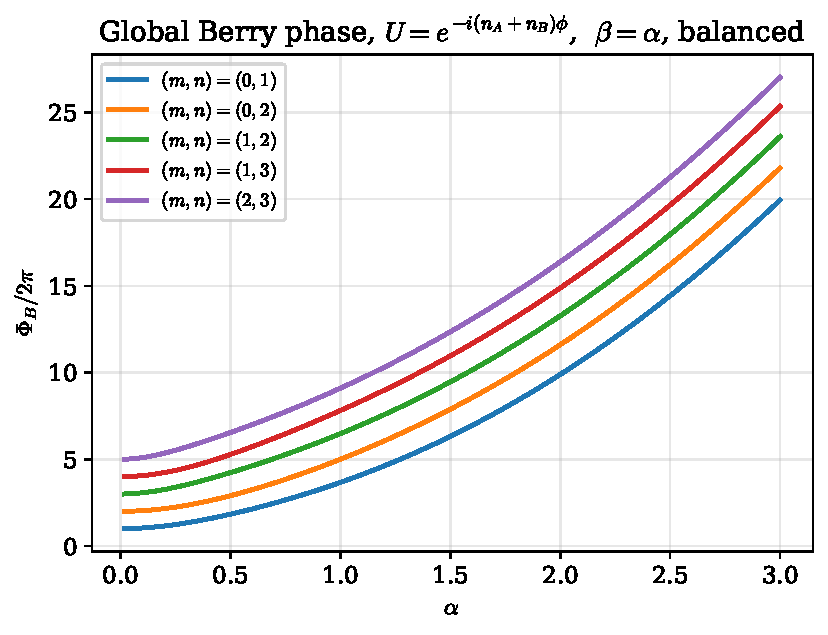
\includegraphics[width=0.66\linewidth]{fig1_berry_global_vs_alpha.pdf}
\caption{Global Berry phase $\Phi_B/2\pi=\langle\nop_A+\nop_B\rangle$,
Eq.~\eqref{eq:berry-global}, versus $\alpha$ for several photon-addition pairs
in the balanced symmetric state. Growth is smooth because the connection is
constant along the cycle; changing $(m,n)$ shifts the curve through both the
diagonal mean-photon terms and the interference term of
Eq.~\eqref{eq:berry-vs-C}.}
\label{fig:f1}\end{figure}

\begin{figure}[htbp]\centering
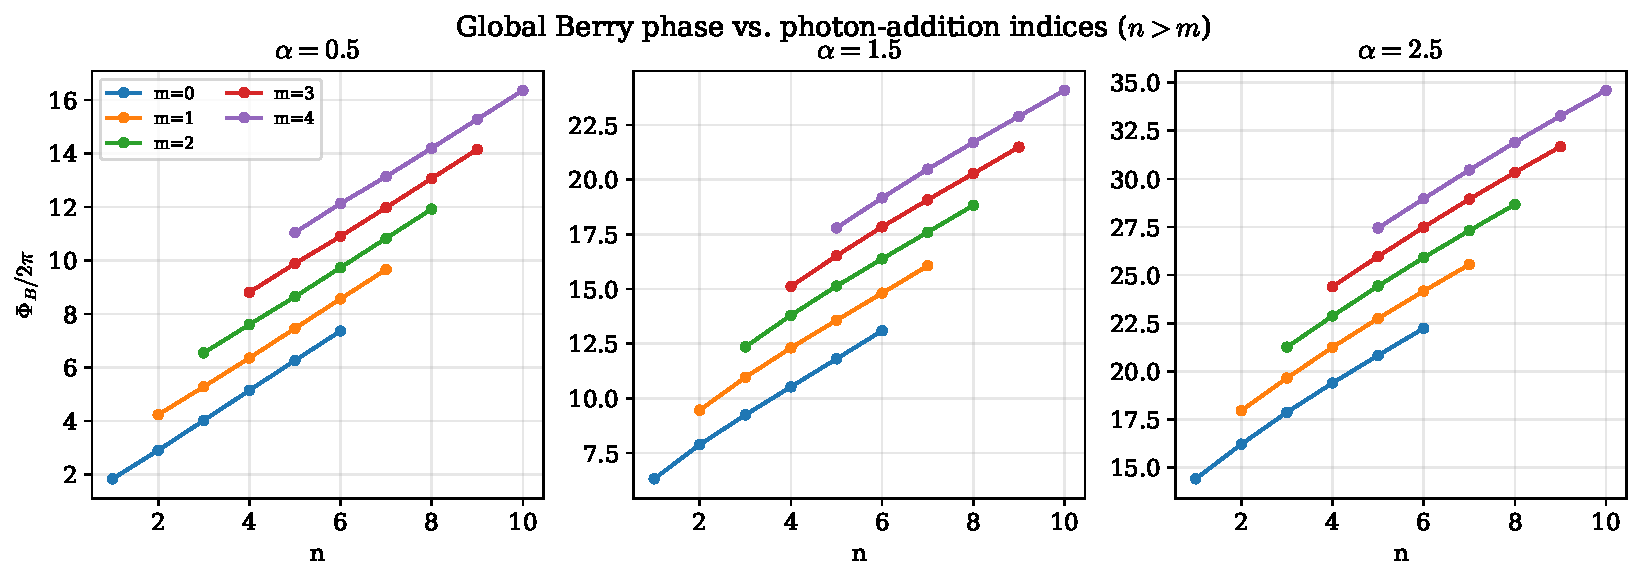
\includegraphics[width=0.98\linewidth]{fig2_berry_global_indices.pdf}
\caption{Discrete dependence of the global Berry phase on the photon-addition
indices at three coherent amplitudes. Only $n>m$ is shown, the ordering in
which the overlap formula \eqref{eq:overlap} is written.}
\label{fig:f2}\end{figure}

\begin{figure}[htbp]\centering
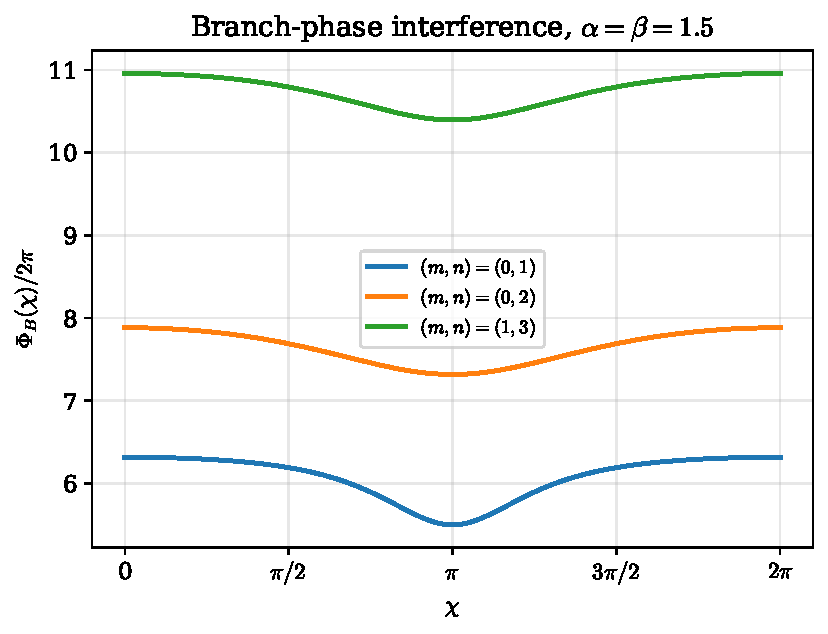
\includegraphics[width=0.66\linewidth]{fig3_berry_global_chi.pdf}
\caption{Interference fringes produced by the tunable relative branch phase
$\chi$. The $\phi$-cycle itself shows no oscillation because its connection,
though containing the coherent cross term, is $\phi$-independent; $\chi$ makes
that interference explicit.}
\label{fig:f3}\end{figure}

\begin{figure}[htbp]\centering
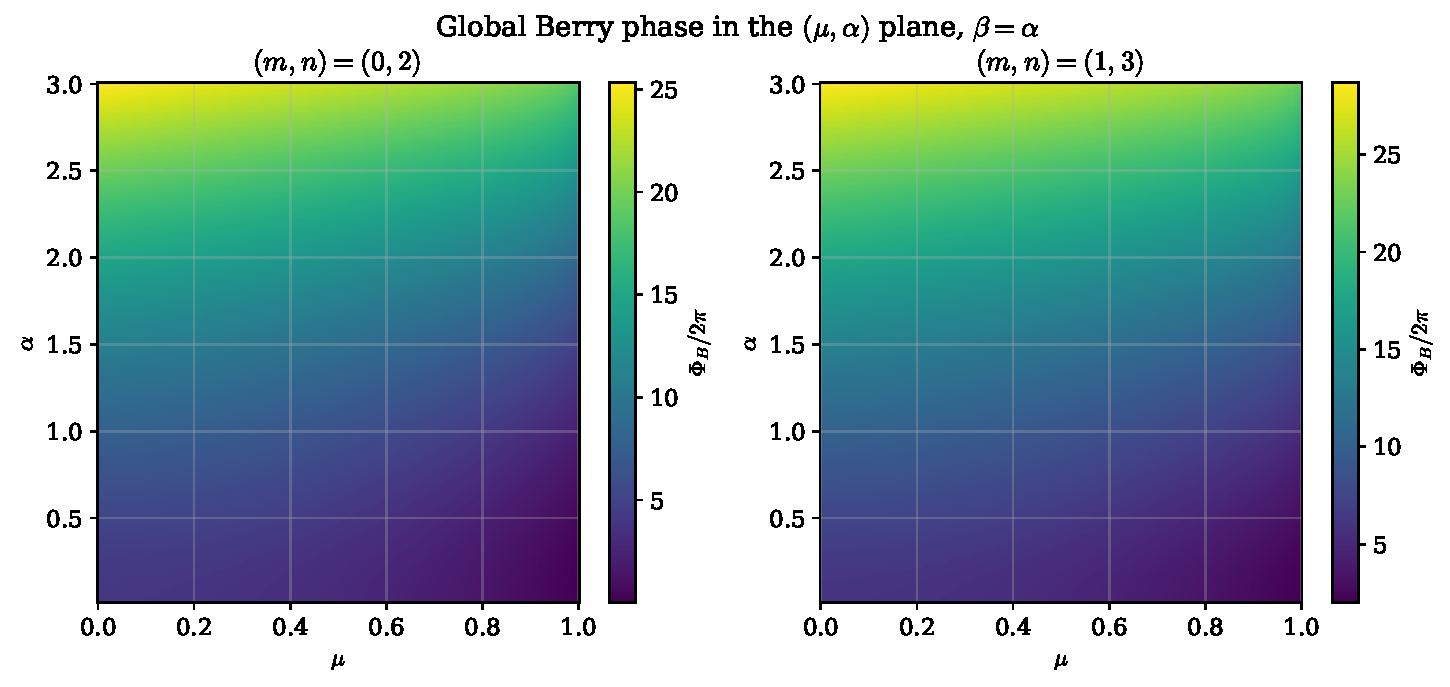
\includegraphics[width=0.95\linewidth]{fig4_berry_global_map.pdf}
\caption{Global Berry phase in the $(\mu,\alpha)$ plane. The map is completely
smooth: a pure-state Berry phase never develops branch cuts, in contrast with
the Uhlmann maps below.}
\label{fig:f4}\end{figure}

\begin{figure}[htbp]\centering
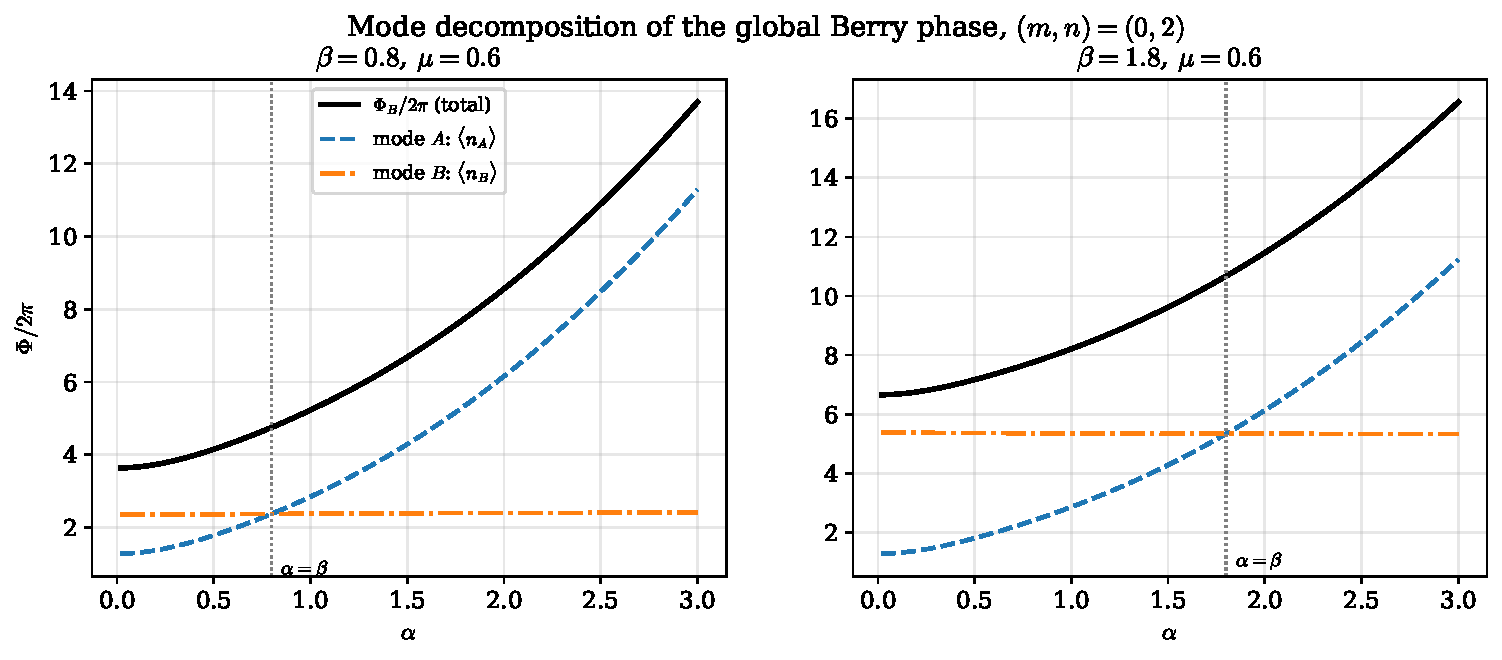
\includegraphics[width=0.95\linewidth]{fig5_berry_mode_decomposition.pdf}
\caption{Exact mode decomposition \eqref{eq:mode-split} of the global Berry
phase for two fixed values of $\beta$. The total (black) is the sum of the two
single-mode contributions; the mode whose amplitude is held fixed contributes
an almost constant amount, so the split is markedly unequal away from
$\alpha=\beta$.}
\label{fig:f5}\end{figure}

\begin{figure}[htbp]\centering
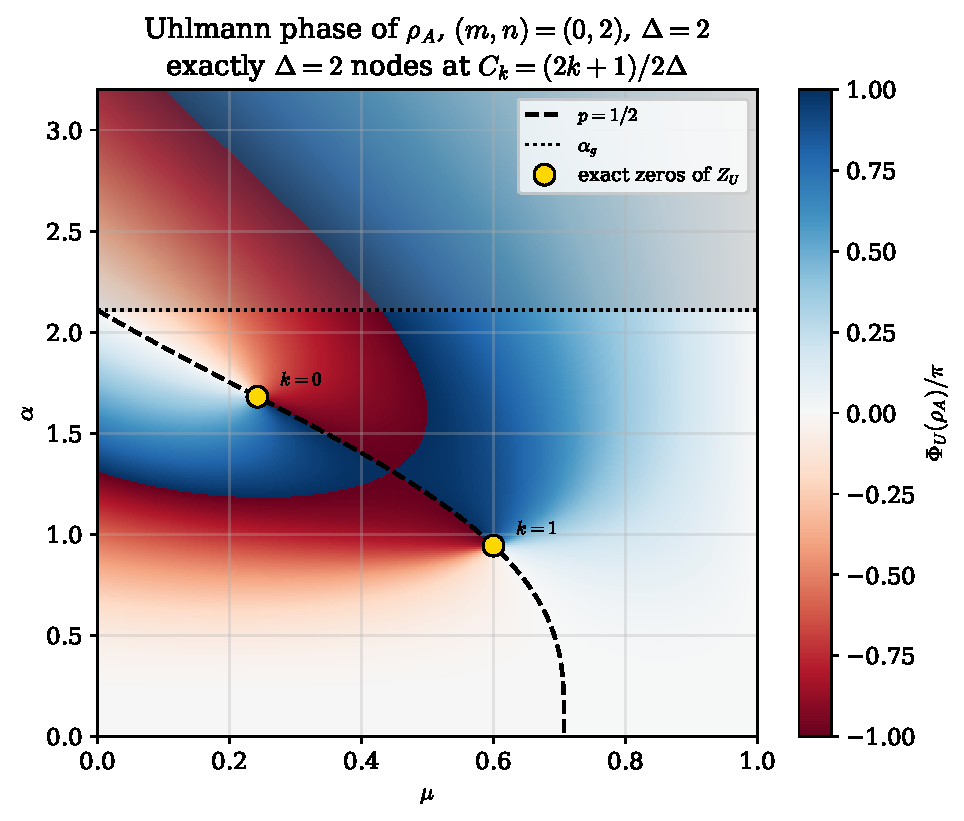
\includegraphics[width=0.68\linewidth]{fig6_uhlmann_map_A.pdf}
\caption{Principal Uhlmann phase of $\rho_A$ in the $(\mu,\alpha)$ plane,
Eq.~\eqref{eq:phiU}, for the symmetric family. The dashed curve is the analytic
condition $p=1/2$, Eq.~\eqref{eq:mu-of-q}; the dotted line is $\alpha_g$ and
the shaded region above it cannot contain nodes. Gold circles are the exact
zeros of $Z_U$: for $\Delta=2$ there are exactly two, labelled $k=0,1$, at
$C_k=(2k+1)/2\Delta$.}
\label{fig:f6}\end{figure}

\begin{figure}[htbp]\centering
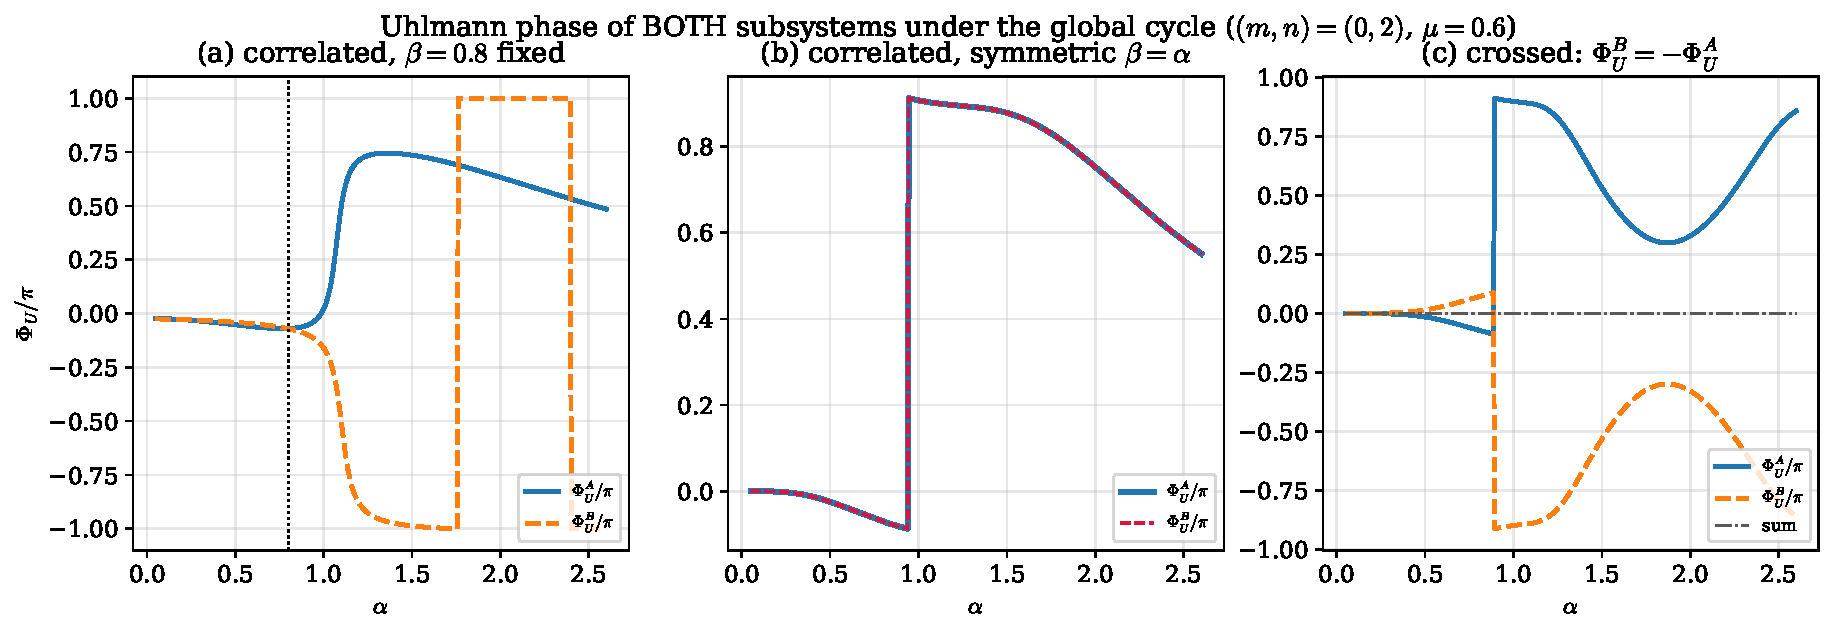
\includegraphics[width=0.99\linewidth]{fig7_uhlmann_both.pdf}
\caption{Uhlmann phase of \emph{both} subsystems under the global cycle.
(a) Branch-correlated family with $\beta=0.8$ fixed: the two phases are
different curves, meeting only at $\alpha=\beta$, even though they share a
concurrence. (b) Symmetric family $\beta=\alpha$: $p_A=p_B$ by
Eq.~\eqref{eq:pApB} and the curves coincide exactly. (c) Crossed family, where
$\omega_B=-\omega_A$: the exact antisymmetry \eqref{eq:antisym} holds and the
sum (dash-dotted) vanishes identically.}
\label{fig:f7}\end{figure}

\begin{figure}[htbp]\centering
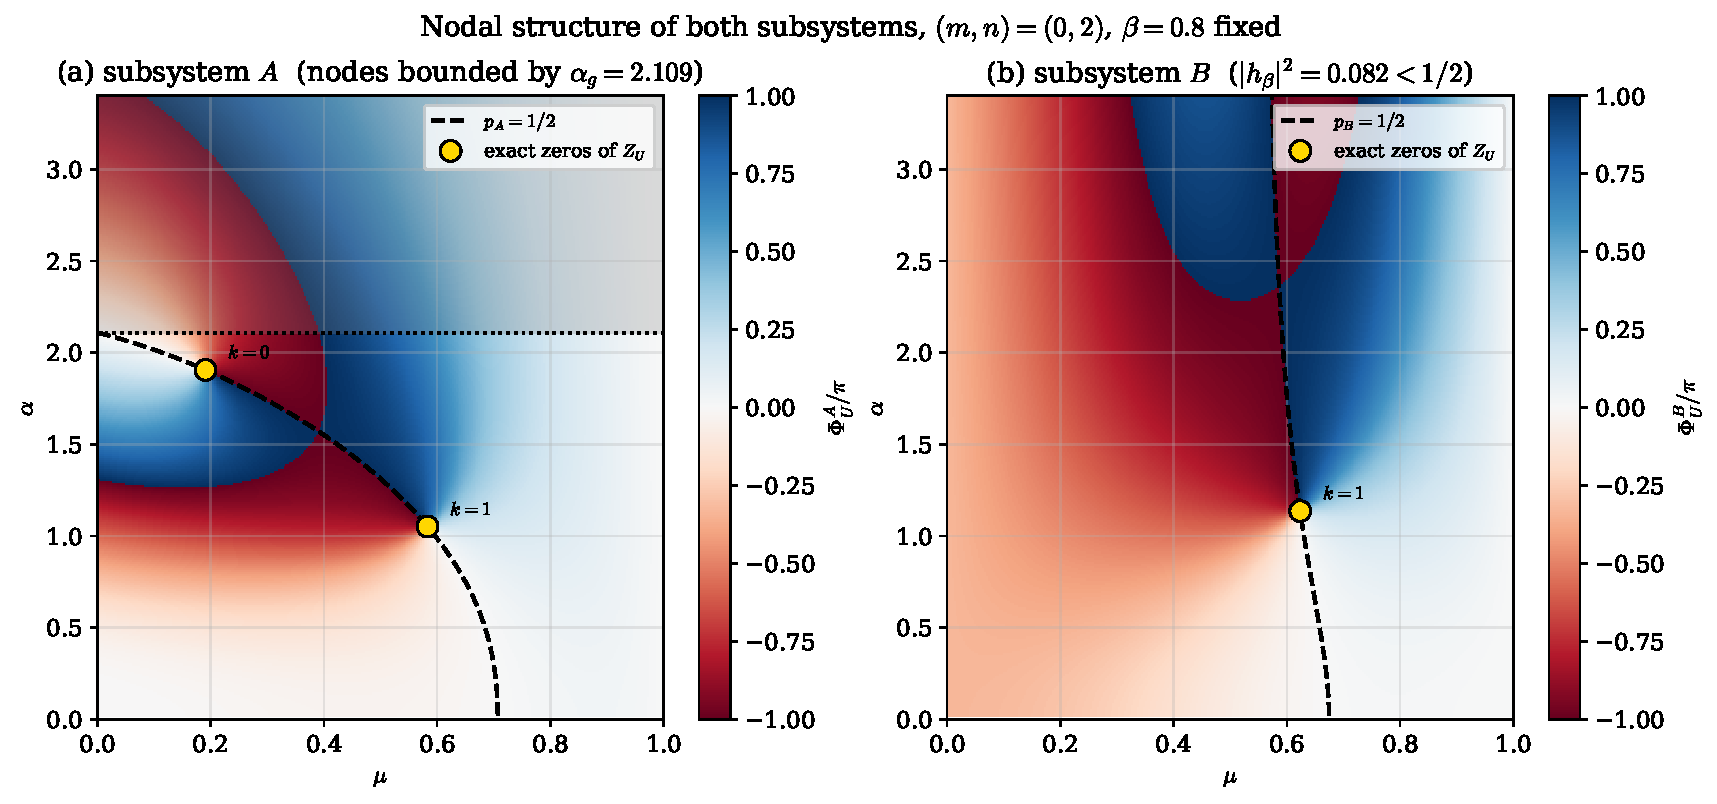
\includegraphics[width=0.99\linewidth]{fig8_nodes_both.pdf}
\caption{Nodal structure of both subsystems in the $(\mu,\alpha)$ plane at
fixed $\beta=0.8$. Both share the same nodal concurrences $C_k$,
Eq.~\eqref{eq:Ck}, but not their coordinates: the $p_A=1/2$ curve bends and
keeps the $A$ nodes below $\alpha_g$, whereas the existence criterion for $B$
depends on $\beta$ alone, so its $p_B=1/2$ curve is nearly vertical and its
nodes are not bounded by $\alpha_g$ (the $k=0$ node of $B$ lies at
$\alpha\approx5.4$, outside the plotted range).}
\label{fig:f8}\end{figure}

\begin{figure}[htbp]\centering
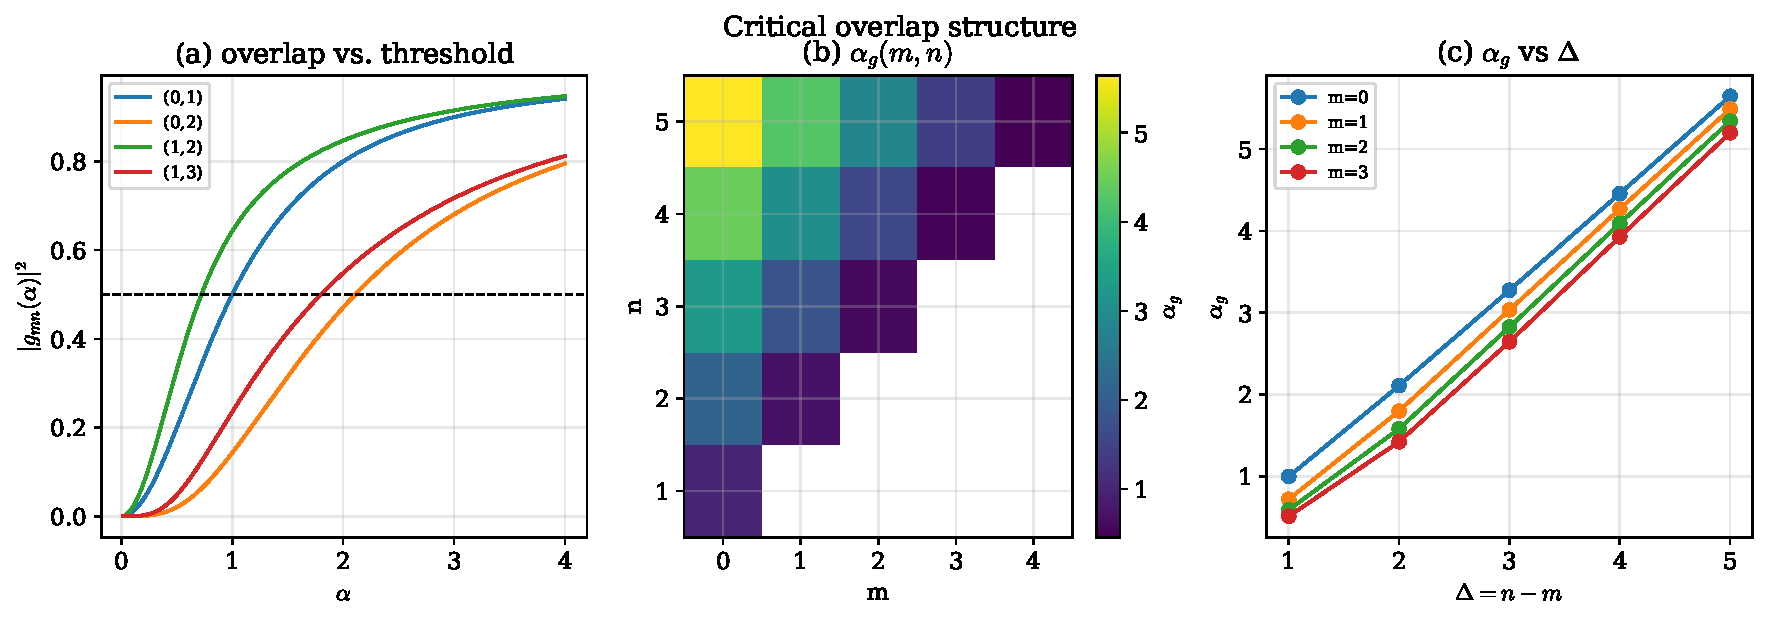
\includegraphics[width=0.98\linewidth]{fig9_critical_overlap.pdf}
\caption{Critical overlap structure. (a) $|g_{mn}(\alpha)|^2$ against the
threshold $1/2$. (b) The discrete critical function $\alpha_g(m,n)$ over the
grid of Table~\ref{tab:alphag}. (c) $\alpha_g$ versus $\Delta$ for several
fixed $m$: larger photon-addition separation extends the nodal region to larger
coherent amplitude.}
\label{fig:f9}\end{figure}

\begin{figure}[htbp]\centering
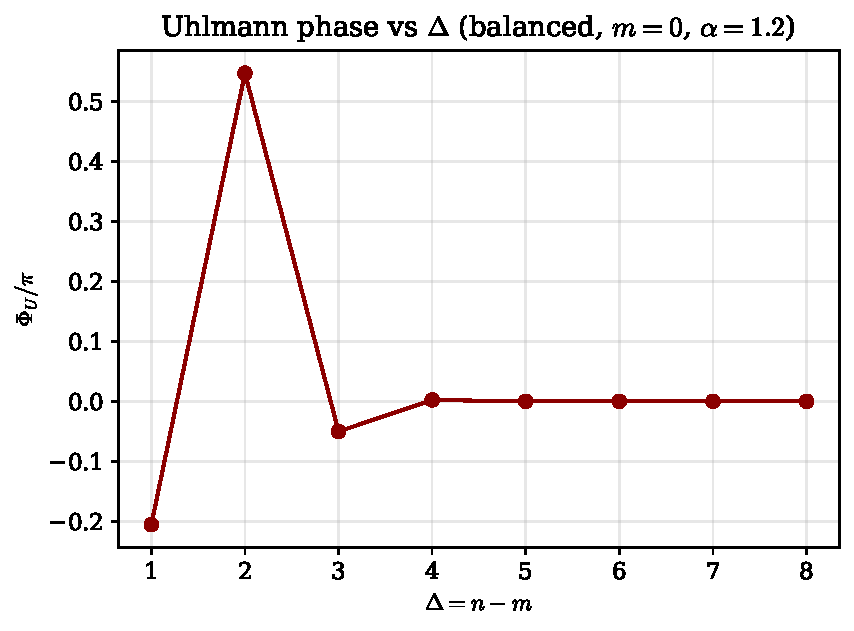
\includegraphics[width=0.66\linewidth]{fig10_uhlmann_vs_Delta.pdf}
\caption{Principal Uhlmann phase versus photon-addition separation $\Delta$ for
the balanced symmetric state. The nonmonotonic behaviour reflects the
dependence of $b=\Delta C$ on $\Delta$ through the overlap, combined with
principal-branch wrapping of $\Arg(\cdot)\in(-\pi,\pi]$.}
\label{fig:f10}\end{figure}

\begin{figure}[htbp]\centering
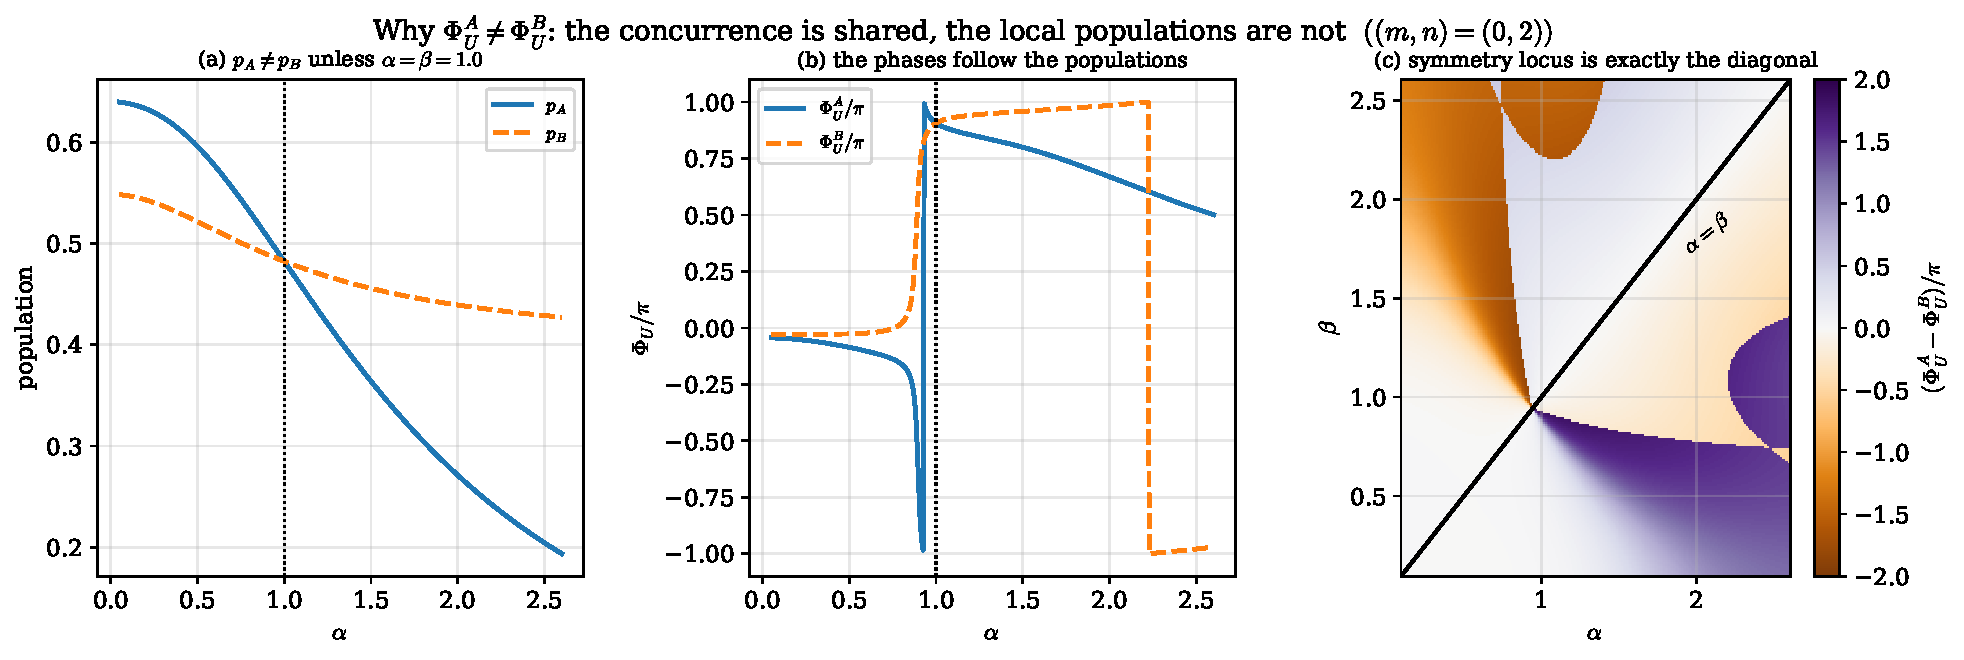
\includegraphics[width=0.99\linewidth]{fig11_AB_asymmetry.pdf}
\caption{Origin of the $A\leftrightarrow B$ asymmetry (Sec.~\ref{sec:asymmetry}).
(a) The local populations differ, crossing only at $\alpha=\beta$. (b) The two
Uhlmann phases track those populations. (c) Map of $\Phi_U^A-\Phi_U^B$ in the
$(\alpha,\beta)$ plane: the symmetry locus is exactly the diagonal
$\alpha=\beta$, where the two local overlaps coincide.}
\label{fig:f11}\end{figure}

\begin{figure}[htbp]\centering
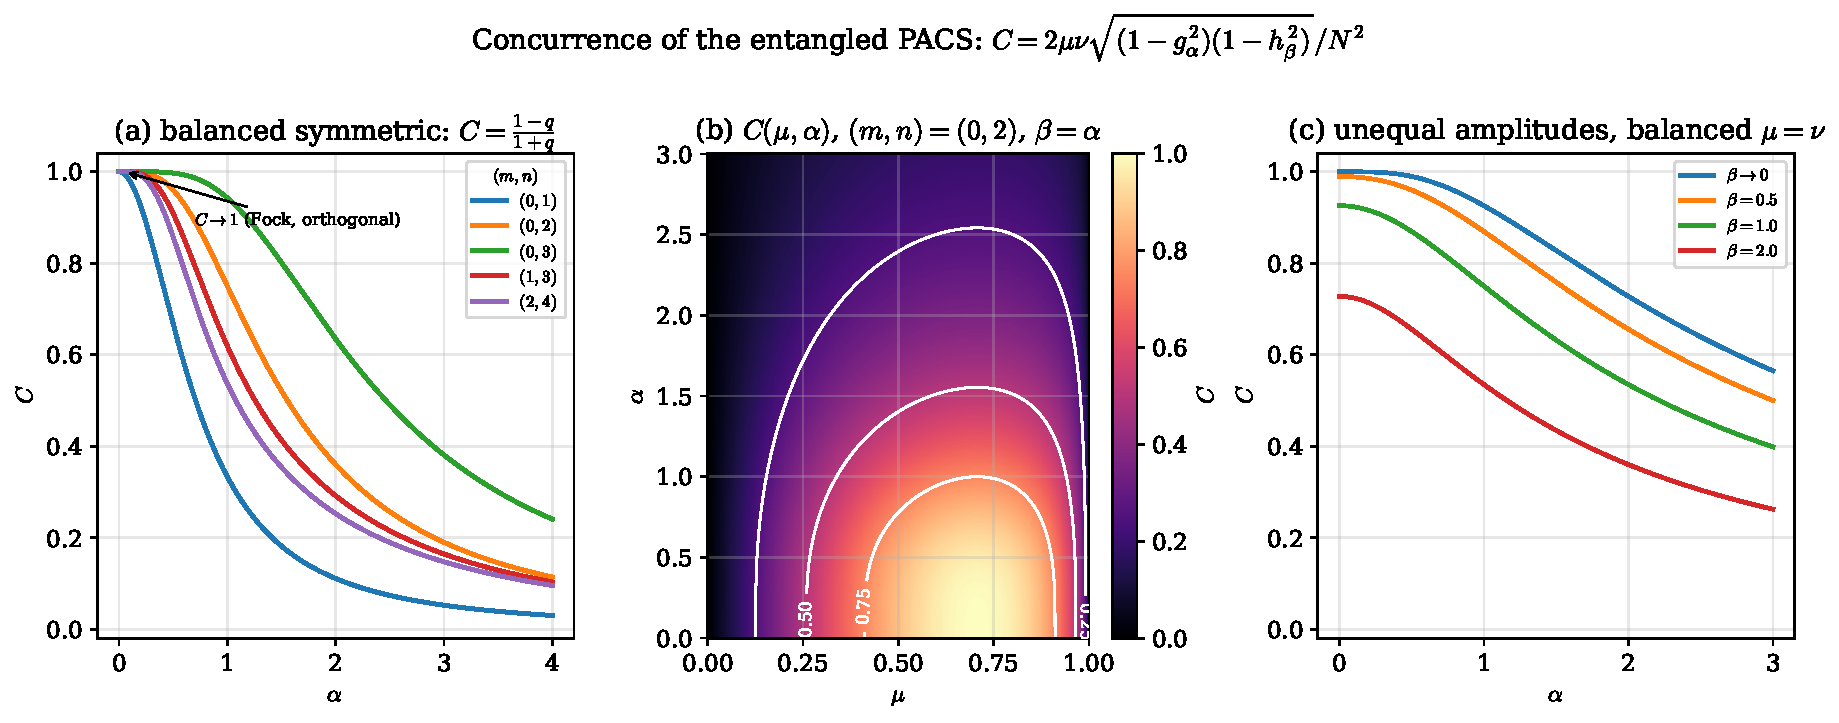
\includegraphics[width=0.99\linewidth]{fig12_concurrence_pacs.pdf}
\caption{Concurrence of the entangled PACS, Eq.~\eqref{eq:concurrence}.
(a) Balanced symmetric family: $C=(1-q)/(1+q)$ decreases monotonically from
$1$ at $\alpha\to0$ (where the PACS reduce to orthogonal Fock states) towards
$0$ at large $\alpha$ (parallel branches). Larger $\Delta$ keeps the branches
distinguishable longer. (b) $C$ over the $(\mu,\alpha)$ plane with contours.
(c) Unequal amplitudes: fixing $\beta$ caps the attainable concurrence, since
$C$ carries the factor $\sqrt{(1-g_\alpha^2)(1-h_\beta^2)}$.}
\label{fig:f12}\end{figure}

\begin{figure}[htbp]\centering
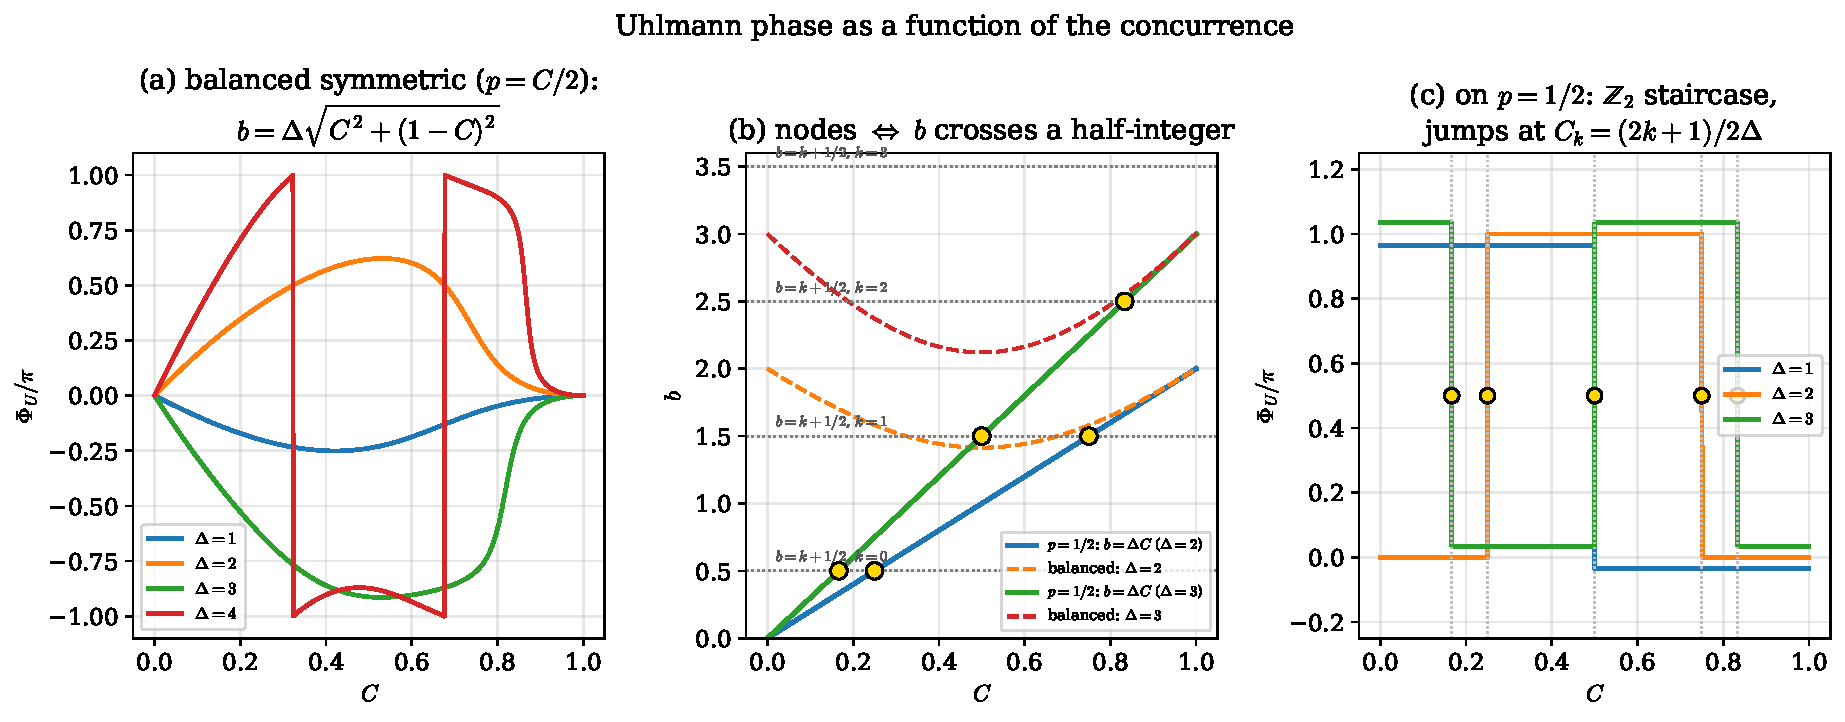
\includegraphics[width=0.99\linewidth]{fig13_uhlmann_vs_concurrence.pdf}
\caption{Uhlmann phase as a function of the concurrence.
(a) In the balanced symmetric family $p=C/2$, so $\Phi_U$ is a pure function of
$C$ through $b=\Delta\sqrt{C^2+(1-C)^2}$, Eq.~\eqref{eq:phiU-of-C}; it returns
to $0$ at both $C=0$ and $C=1$. (b) $b$ versus $C$ on the two loci, with the
half-integer levels dotted: on $p=1/2$ the line $b=\Delta C$ crosses them
exactly at the nodal concurrences (gold). The balanced curve may also cross a
half-integer, but those are not nodes because $p\neq1/2$ leaves
$\mathrm{Im}\,Z_U\neq0$. (c) On $p=1/2$ the phase is the $\mathbb{Z}_2$
staircase of Eq.~\eqref{eq:Z2}, flipping between $0$ and $\pi$ exactly at the
$\Delta$ nodal concurrences (curves offset vertically for visibility).}
\label{fig:f13}\end{figure}

\begin{figure}[htbp]\centering
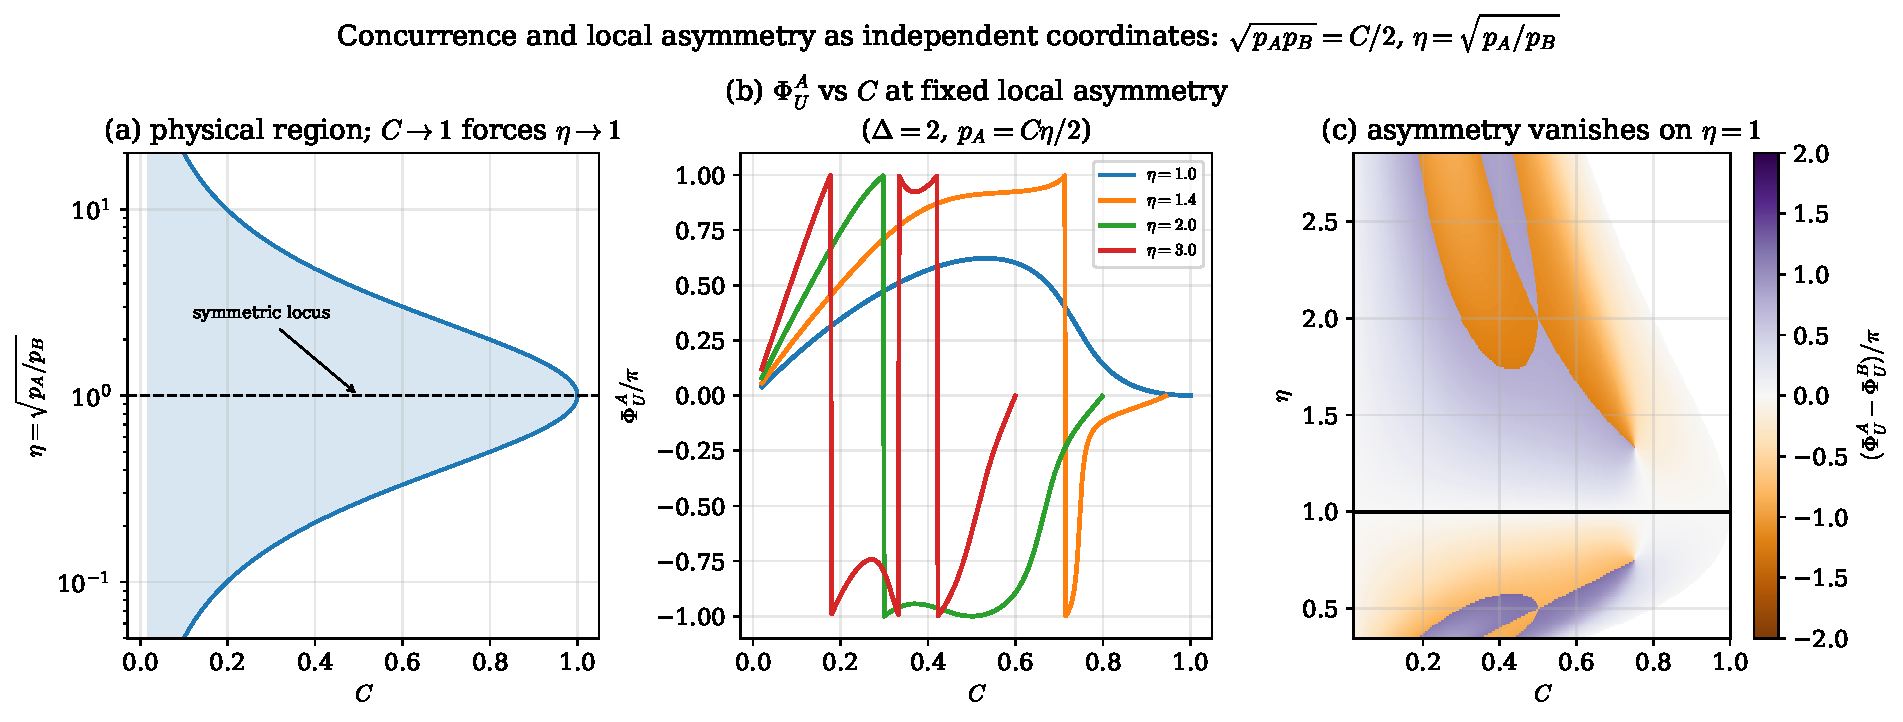
\includegraphics[width=0.99\linewidth]{fig14_C_eta_plane.pdf}
\caption{Concurrence and local asymmetry as independent coordinates,
Eqs.~\eqref{eq:geometric-mean}--\eqref{eq:eta}. (a) The physical region
\eqref{eq:eta-range} in the $(C,\eta)$ plane; it is symmetric under
$\eta\to1/\eta$ and pinches to the single point $\eta=1$ as $C\to1$, so maximal
entanglement enforces $A\leftrightarrow B$ symmetry. (b) $\Phi_U^A$ versus $C$
at fixed local asymmetry $\eta$. (c) $\Phi_U^A-\Phi_U^B$ over the same plane:
the asymmetry vanishes identically on the line $\eta=1$.}
\label{fig:f14}\end{figure}

\begin{figure}[htbp]\centering
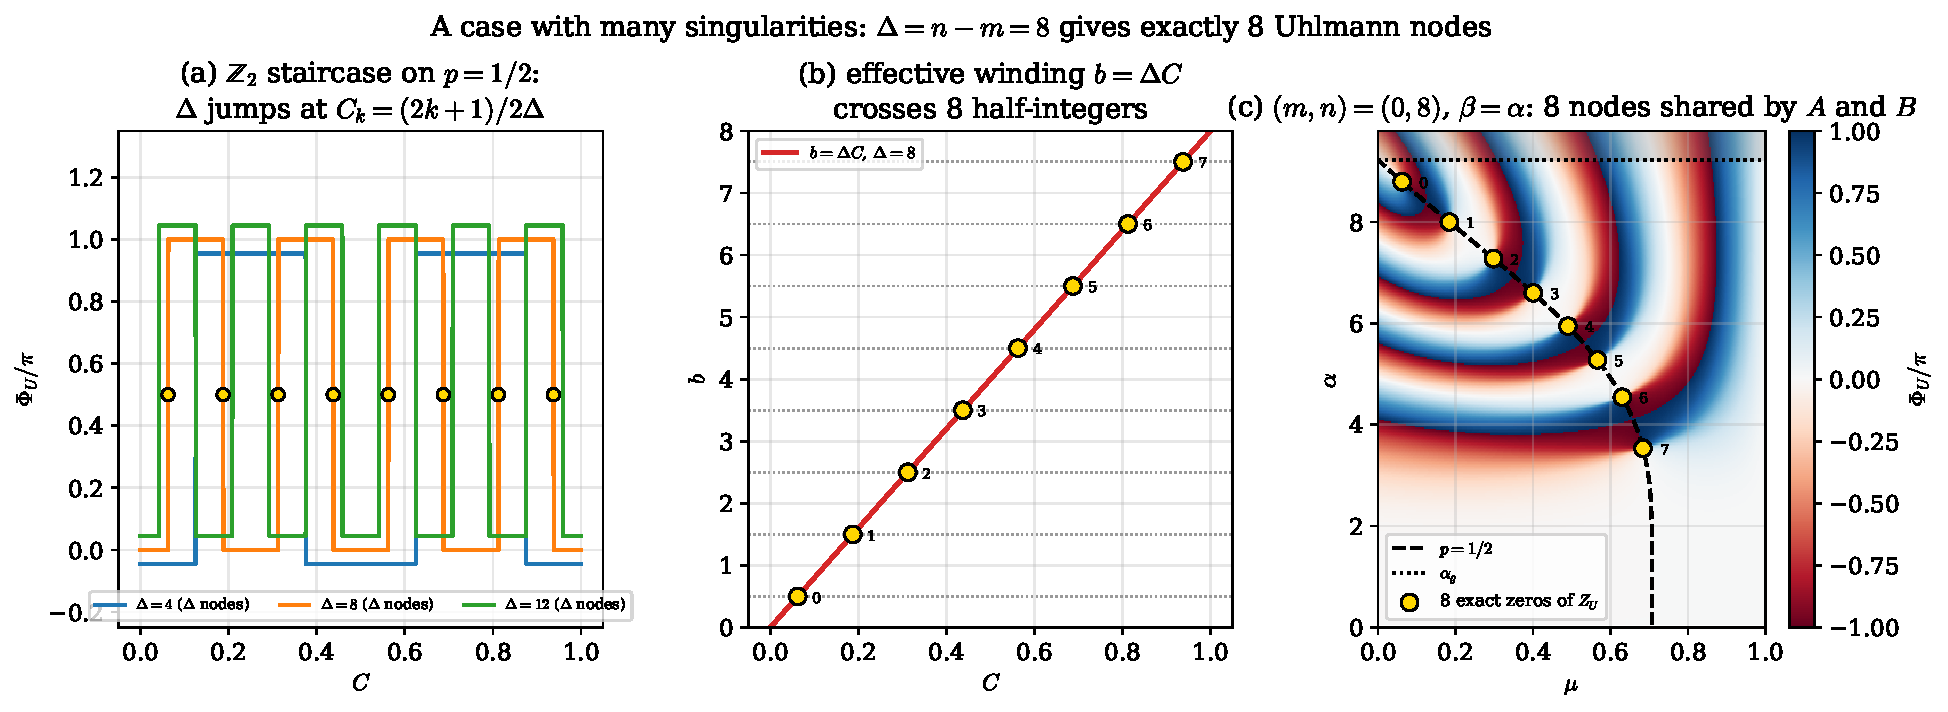
\includegraphics[width=0.99\linewidth]{fig15_many_nodes.pdf}
\caption{A case with many singularities, $\Delta=n-m=8$. (a) The
$\mathbb{Z}_2$ staircase of Eq.~\eqref{eq:Z2} now takes $\Delta$ steps;
curves for $\Delta=4,8,12$ are offset vertically. (b) The effective winding
$b=\Delta C$ crosses $\Delta=8$ half-integers, one per node (gold, labelled by
$k$). (c) The eight nodes in the $(\mu,\alpha)$ plane for the symmetric family
$\beta=\alpha$, strung along the $p=1/2$ curve and all below
$\alpha_g=9.23$; since $p_A=p_B$ there, these eight points are the nodes of
\emph{both} subsystems.}
\label{fig:f15}\end{figure}

\begin{figure}[htbp]\centering
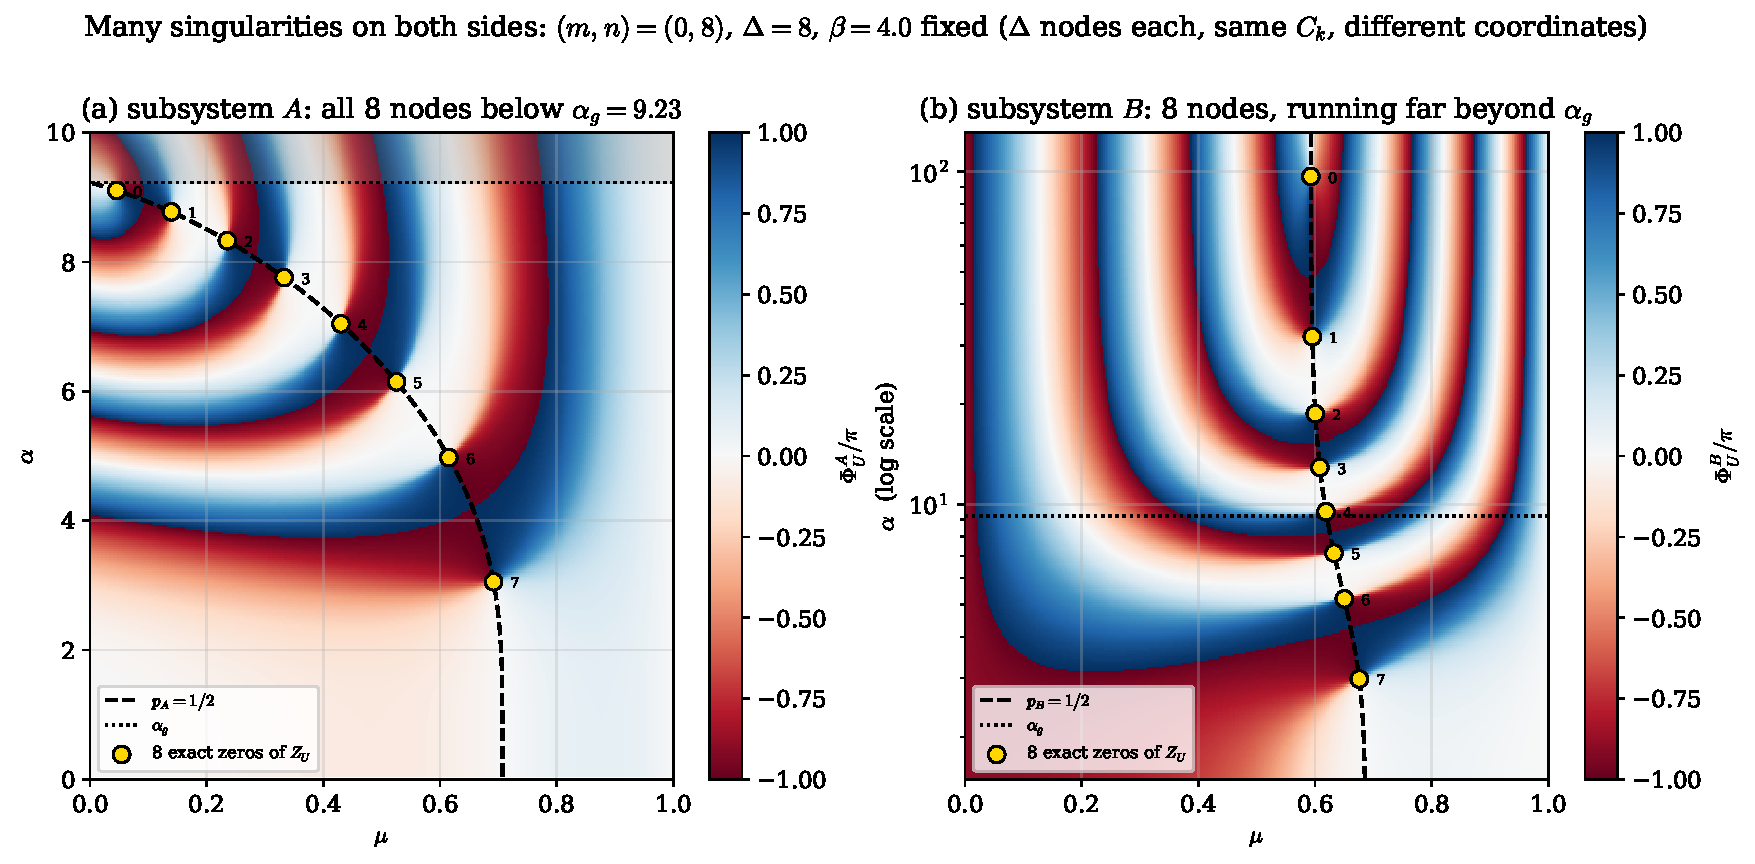
\includegraphics[width=0.99\linewidth]{fig16_many_nodes_AB.pdf}
\caption{The same $\Delta=8$ case with $\beta=4$ fixed, so that the two
subsystems separate. Each side still carries exactly eight nodes at the same
concurrences $C_k$, but at wildly different coordinates: (a) the eight nodes of
$A$ all lie below $\alpha_g=9.23$ (shaded region excluded); (b) those of $B$,
bounded only by the criterion \eqref{eq:B-existence} on $\beta$, run out to
$\alpha\approx97$ --- note the logarithmic $\alpha$ axis. Numerical values in
Table~\ref{tab:many}.}
\label{fig:f16}\end{figure}

\begin{figure}[htbp]\centering
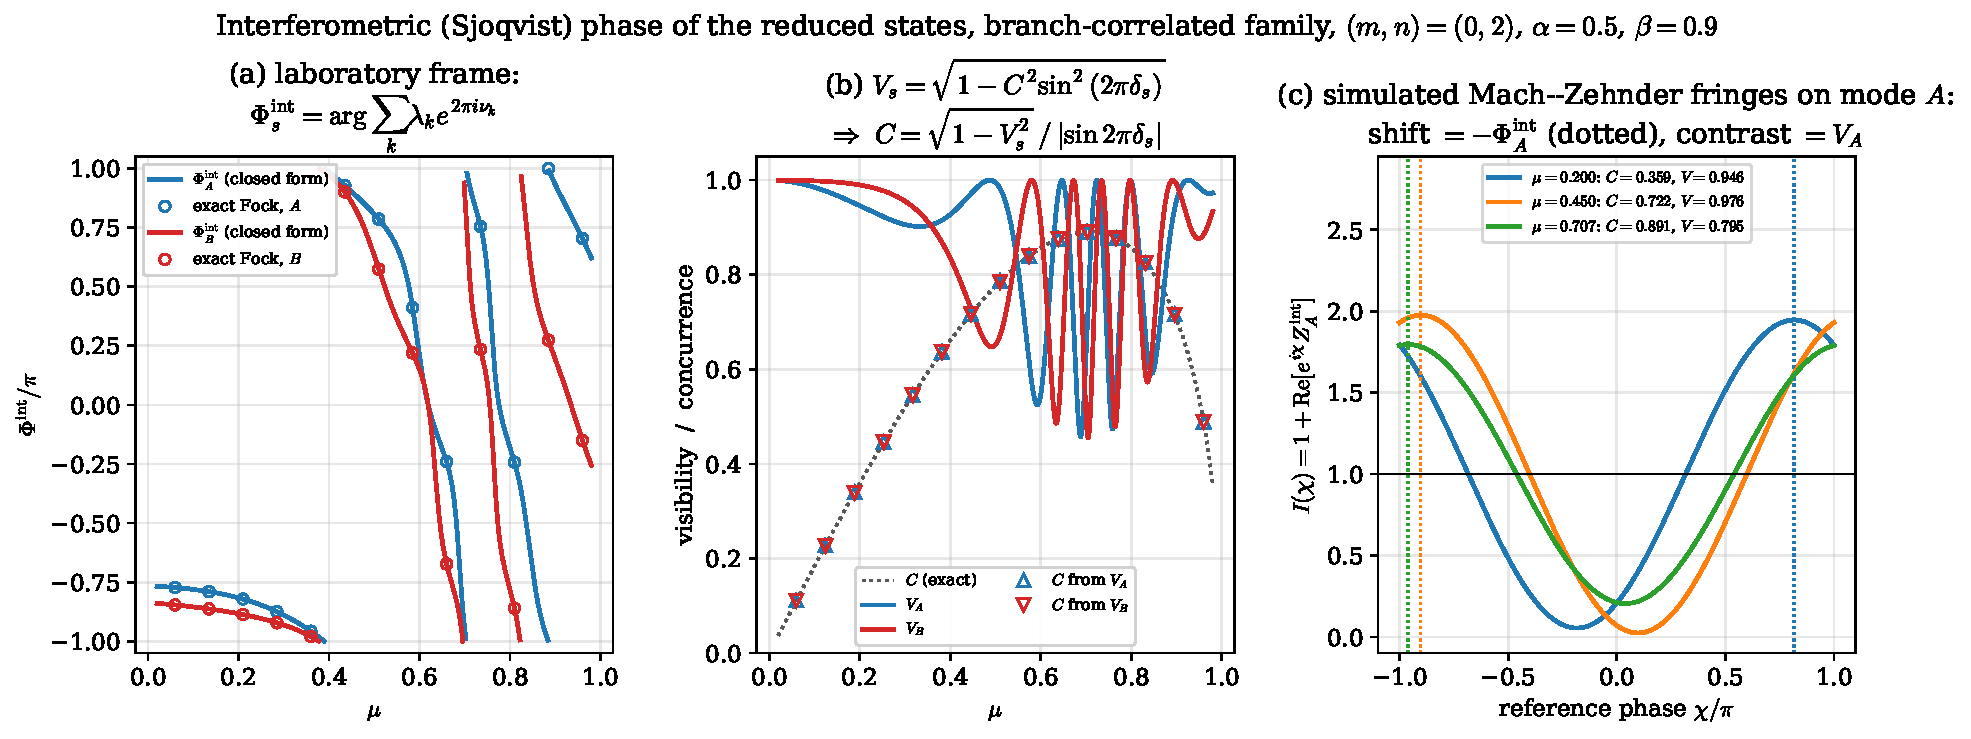
\includegraphics[width=0.99\linewidth]{fig17_interferometric_lab.pdf}
\caption{Interferometric (Sj\"oqvist) phase of the two reduced states in the
laboratory frame, Eqs.~\eqref{eq:int-lab}--\eqref{eq:int-lab-closed}, for the
branch-correlated family with $(m,n)=(0,2)$, $\alpha=0.5$, $\beta=0.9$.
(a) $\Phi^{\rm int}_A$ and $\Phi^{\rm int}_B$ versus $\mu$: lines are the
closed form, markers the exact truncated-Fock evaluation of
$\Arg\sum_k\lambda_ke^{2\pi i\nu_k}$ (agreement $4\times10^{-14}$). The two
subsystems differ because the offsets $\pi\Tr\mathcal N_s$ and the splittings
$\delta_s$ are local properties of each mode.
(b) Fringe contrast $\mathcal V_s=\sqrt{1-C^2\sin^2 2\pi\delta_s}$ (solid)
against the exact concurrence (dotted); triangles are the concurrence
\emph{reconstructed} from the contrast of a single mode through the witness
\eqref{eq:witness}, and fall on the exact curve.
(c) Simulated Mach--Zehnder fringes $I(\chi)=1+\mathrm{Re}[e^{i\chi}Z^{\rm int}_A]$
at three values of $\mu$: the fringe shift is $-\Phi^{\rm int}_A$ (dotted
verticals) and the contrast is $\mathcal V_A$.}
\label{fig:f17}\end{figure}

\begin{figure}[htbp]\centering
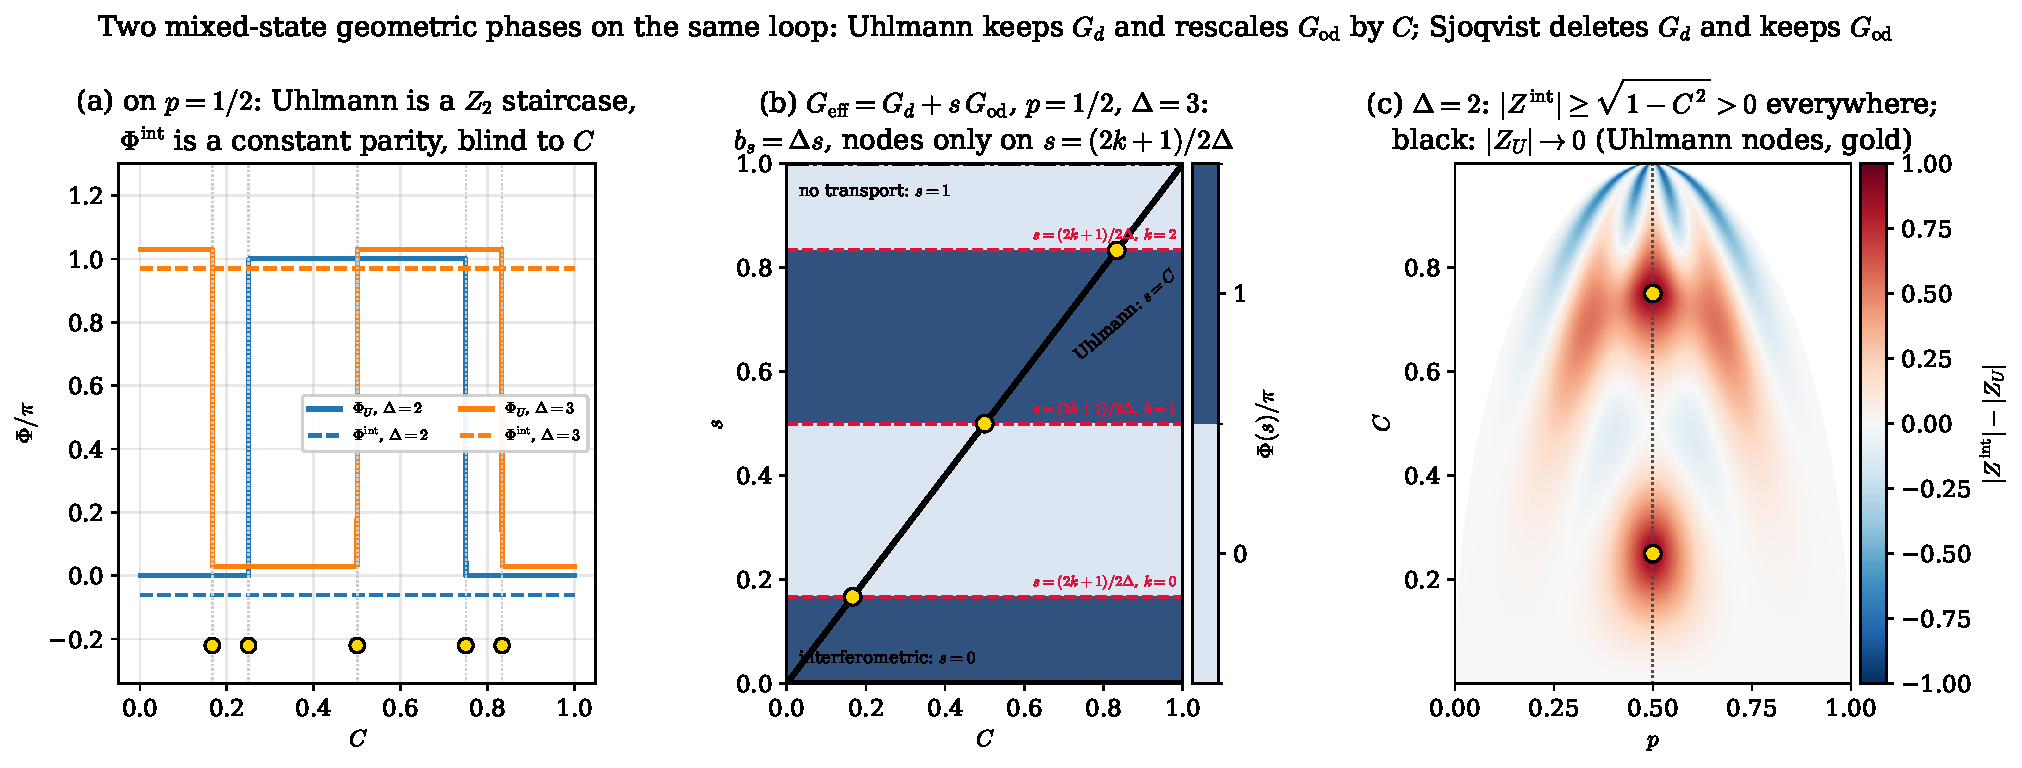
\includegraphics[width=0.99\linewidth]{fig18_interf_vs_uhlmann.pdf}
\caption{The two mixed-state geometric phases on the same logical loop,
Eq.~\eqref{eq:two-transports}.
(a) On $p=1/2$: the Uhlmann phase is the $\mathbb Z_2$ staircase of
Eq.~\eqref{eq:Z2}, jumping at the quantized concurrences
$C_k=(2k+1)/2\Delta$ (gold), while the interferometric phase is the constant
parity $\pi\Delta$ of Eq.~\eqref{eq:int-half}, blind to $C$ (curves offset
vertically for legibility).
(b) The interpolating family $G_{\rm eff}=G_d+s\,G_{\rm od}$ of
Eq.~\eqref{eq:Zs} at $p=1/2$, $\Delta=3$: since $b_s=\Delta s$, all nodes lie
on the horizontal lines $s=(2k+1)/2\Delta$ (dashed). The Uhlmann phase runs
along the diagonal $s=C$ and meets every one of them; the interferometric
phase runs along $s=0$ and meets none; $s=1$ is the untransported cycle.
(c) Difference of moduli over the physical region $(p,C)$ for $\Delta=2$:
$|Z^{\rm int}|\geq\sqrt{1-C^2}>0$ everywhere, whereas $|Z_U|$ vanishes at the
two gold nodes on $p=1/2$ (black contour $|Z_U|=0.02$).}
\label{fig:f18}\end{figure}

\begin{figure}[htbp]\centering
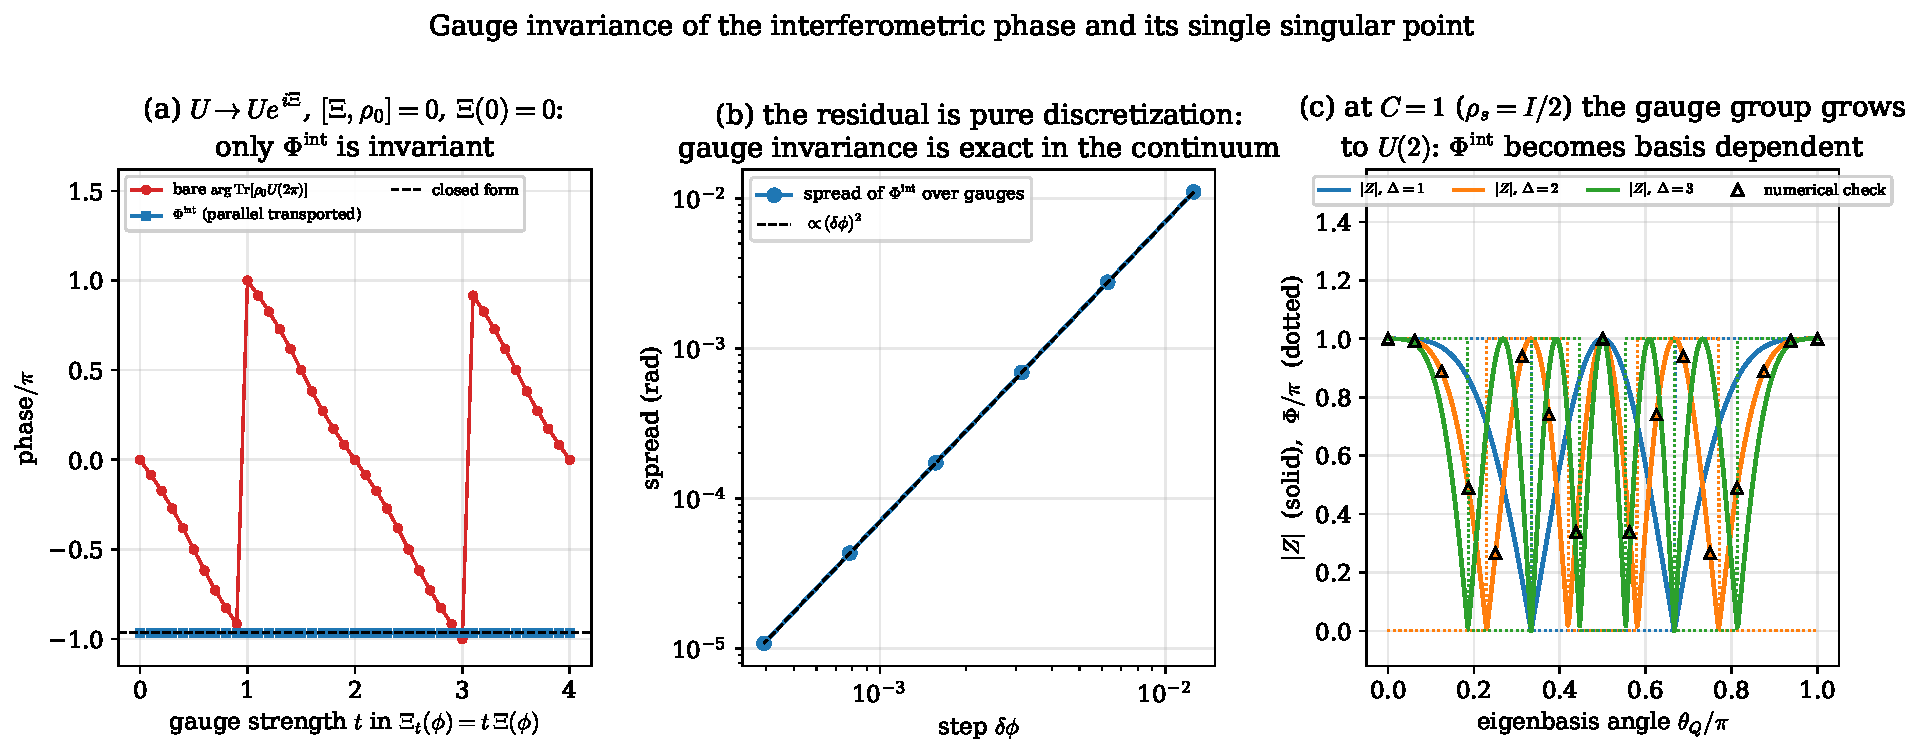
\includegraphics[width=0.99\linewidth]{fig19_gauge_invariance.pdf}
\caption{Gauge invariance of the interferometric phase, Sec.~\ref{sec:int-gauge}.
(a) Under the one-parameter gauge family $U\to Ue^{i t\Xi(\phi)}$ with
$[\Xi,\rho_0]=0$ and $\Xi(0)=0$, the bare Pancharatnam phase
$\Arg\Tr[\rho_0U(2\pi)]$ sweeps the entire circle while $\Phi^{\rm int}$ stays
pinned to the closed form \eqref{eq:int-log} (dashed).
(b) The residual spread of $\Phi^{\rm int}$ over gauges scales as
$(\delta\phi)^2$: gauge invariance is exact in the continuum and the residual
is purely the discretization of the transport integral.
(c) At $C=1$, where $\rho_s=\mathbb 1/2$ and the gauge group grows to $U(2)$,
the phase becomes basis dependent: $|Z^{\rm int}|=|\cos(\pi\Delta\cos\theta_Q)|$
as a function of the eigenbasis angle, Eq.~\eqref{eq:degenerate}, with zeros
whenever $\Delta\cos\theta_Q$ is a half-integer (triangles: direct numerical
evaluation of Eq.~\eqref{eq:int-holonomy}).}
\label{fig:f19}\end{figure}

\begin{table}[htbp]\centering
\caption{Critical amplitudes $\alpha_g(m,n)$ from $|g_{mn}(\alpha_g)|^2=1/2$.}
\label{tab:alphag}
\begin{tabular}{c|ccccc}
\toprule
$n\backslash m$ & 0 & 1 & 2 & 3 & 4\\
\midrule
1 & 1.0000 & & & & \\
2 & 2.1094 & 0.7221 & & & \\
3 & 3.2756 & 1.8000 & 0.5921 & & \\
4 & 4.4576 & 3.0354 & 1.5829 & 0.5135 & \\
5 & 5.6464 & 4.2685 & 2.8269 & 1.4235 & 0.4596\\
\bottomrule
\end{tabular}
\end{table}

\begin{table}[htbp]\centering
\caption{Complete Uhlmann nodal set, Eqs.~\eqref{eq:Ck}--\eqref{eq:nodal-coords}.
Each $\Delta$ supports exactly $\Delta$ nodes; all satisfy $p=1/2$ and
$\alpha_k<\alpha_g$. The last column is the numerically evaluated $|Z_U|$.}
\label{tab:nodes}
\begin{tabular}{cccccccc}
\toprule
$(m,n)$ & $\Delta$ & $k$ & $C_k$ & $\mu_k$ & $\alpha_k$ & $\alpha_g$ & $|Z_U|$\\
\midrule
$(0,1)$ & 1 & 0 & 0.5000 & 0.4472 & 0.5774 & 1.0000 & $4.5\times10^{-16}$\\
\midrule
$(0,2)$ & 2 & 0 & 0.2500 & 0.2425 & 1.6807 & 2.1094 & $6.1\times10^{-17}$\\
        &   & 1 & 0.7500 & 0.6000 & 0.9444 & 2.1094 & $1.8\times10^{-16}$\\
\midrule
$(0,3)$ & 3 & 0 & 0.1667 & 0.1644 & 2.8433 & 3.2756 & $3.4\times10^{-15}$\\
        &   & 1 & 0.5000 & 0.4472 & 2.1094 & 3.2756 & $1.8\times10^{-16}$\\
        &   & 2 & 0.8333 & 0.6402 & 1.3628 & 3.2756 & $2.1\times10^{-15}$\\
\midrule
$(1,2)$ & 1 & 0 & 0.5000 & 0.4472 & 0.4095 & 0.7221 & $5.7\times10^{-15}$\\
\midrule
$(1,3)$ & 2 & 0 & 0.2500 & 0.2425 & 1.3763 & 1.8000 & $6.1\times10^{-17}$\\
        &   & 1 & 0.7500 & 0.6000 & 0.7265 & 1.8000 & $6.6\times10^{-14}$\\
\midrule
$(1,4)$ & 3 & 0 & 0.1667 & 0.1644 & 2.5872 & 3.0354 & $5.5\times10^{-15}$\\
        &   & 1 & 0.5000 & 0.4472 & 1.8378 & 3.0354 & $5.0\times10^{-15}$\\
        &   & 2 & 0.8333 & 0.6402 & 1.1224 & 3.0354 & $2.4\times10^{-15}$\\
\midrule
$(2,4)$ & 2 & 0 & 0.2500 & 0.2425 & 1.1867 & 1.5829 & $3.1\times10^{-15}$\\
        &   & 1 & 0.7500 & 0.6000 & 0.6130 & 1.5829 & $1.8\times10^{-16}$\\
\bottomrule
\end{tabular}
\end{table}

\begin{table}[htbp]\centering
\caption{Interferometric phases of both subsystems. $\Phi^{\rm int}_s/\pi$ is the
laboratory-frame phase \eqref{eq:int-lab}, evaluated by direct diagonalization
of the exact truncated-Fock $\rho_s(0)$; it agrees with the closed form
\eqref{eq:int-lab-closed} to $4\times10^{-14}$ on every row.
$C(\mathcal V_s)$ is the concurrence reconstructed from the single-mode fringe
contrast through the witness \eqref{eq:witness}; it reproduces the exact $C$ to
$3\times10^{-14}$. The last two columns give the interferometric and Uhlmann
phases of the same logical loop, Eqs.~\eqref{eq:int-log} and \eqref{eq:phiU},
for comparison: note the exact antisymmetry between $A$ and $B$ in the crossed
family, and its absence in the laboratory frame.}
\label{tab:interf}
\footnotesize
\setlength{\tabcolsep}{3.2pt}
\begin{tabular}{llccccccccccc}
\toprule
family & $(m,n)$ & $\alpha$ & $\beta$ & $\mu$ & $s$ & $C$ & $\delta_s$ &
$\Phi^{\rm int}_s/\pi$ & $\mathcal V_s$ & $C(\mathcal V_s)$ &
$\Phi^{\rm int,log}_s/\pi$ & $\Phi_U^{\rm log}/\pi$\\
\midrule
corr. & $(0,2)$ & 0.5 & 0.9 & 0.4500 & $A$ & 0.7223 & +1.0489 & +0.9021 & 0.9759 & 0.7223 & -0.5578 & -0.1551\\
 &  &  &  &  & $B$ & 0.7223 & +1.2923 & +0.8577 & 0.7172 & 0.7223 & -0.9610 & -0.2727\\
\midrule
corr. & $(0,2)$ & 0.5 & 0.9 & 0.7071 & $A$ & 0.8906 & +0.1190 & +0.9604 & 0.7956 & 0.8906 & -0.1650 & +0.0184\\
 &  &  &  &  & $B$ & 0.8906 & +0.2305 & +0.6539 & 0.4677 & 0.8906 & -0.7882 & +0.0369\\
\midrule
corr. & $(0,2)$ & 1.1 & 0.8 & 0.6000 & $A$ & 0.7480 & +0.8099 & +0.7985 & 0.7183 & 0.7480 & -0.1158 & +0.4987\\
 &  &  &  &  & $B$ & 0.7480 & +0.6992 & -0.8057 & 0.7040 & 0.7480 & +0.1104 & -0.5034\\
\midrule
corr. & $(1,3)$ & 1.3 & 0.7 & 0.4500 & $A$ & 0.5257 & +1.1058 & -0.7164 & 0.9460 & 0.5257 & -0.2219 & +0.9856\\
 &  &  &  &  & $B$ & 0.5257 & +0.9245 & -0.1837 & 0.9708 & 0.5257 & +0.5100 & -0.9450\\
\midrule
corr. & $(2,4)$ & 0.8 & 1.6 & 0.3500 & $A$ & 0.3373 & +1.0136 & +0.8698 & 0.9996 & 0.3373 & +0.2841 & +0.8699\\
 &  &  &  &  & $B$ & 0.3373 & +1.1967 & +0.3783 & 0.9479 & 0.3373 & -0.6096 & -0.9219\\
\midrule
cross. & $(0,2)$ & 1.1 & 0.8 & 0.6000 & $A$ & 0.5574 & +0.7078 & -0.5238 & 0.8430 & 0.5574 & -0.6400 & +0.8892\\
 &  &  &  &  & $B$ & 0.5574 & +0.1424 & +0.3322 & 0.9005 & 0.5574 & +0.6400 & -0.8892\\
\midrule
cross. & $(0,3)$ & 1.5 & 1.2 & 0.5000 & $A$ & 0.5972 & +1.3190 & +0.3278 & 0.8404 & 0.5972 & -0.8948 & +0.9862\\
 &  &  &  &  & $B$ & 0.5972 & -0.5687 & +0.5484 & 0.9683 & 0.5972 & +0.8948 & -0.9862\\
\midrule
cross. & $(0,1)$ & 0.9 & 0.9 & 0.7071 & $A$ & 0.3817 & +0.3345 & -0.6999 & 0.9443 & 0.3817 & +0.3199 & +0.2478\\
 &  &  &  &  & $B$ & 0.3817 & +0.3345 & -0.6999 & 0.9443 & 0.3817 & -0.3199 & -0.2478\\
\bottomrule
\end{tabular}
\end{table}

% =========================================================================
\section{Discussion}
% =========================================================================

Choosing the global cycle organizes the problem into three clean levels.

\emph{Level 1 --- the connection is a photon number.} Because
$\nop_A+\nop_B$ generates the cycle and commutes with itself, the Berry
connection is constant and equals the total mean photon number. Everything in
the Berry sector is therefore smooth, single-valued and additive across modes,
Eq.~\eqref{eq:mode-split}. The interference between branches is present in the
connection but invisible in $\phi$; it takes a separately controllable branch
phase to expose it.

\emph{Level 2 --- entanglement enters affinely.} In the balanced symmetric
family the global Berry phase is an affine function of the concurrence,
Eq.~\eqref{eq:berry-vs-C}, interpolating between a mean-photon average and a
pure interference term. This is as far as a pure-state geometric phase can go:
it cannot be singular.

\emph{Level 3 --- mixed-state holonomy, and it has two sides.} Tracing out
either mode leaves a genuinely mixed state, and the Uhlmann holonomy can be
singular. The compact result \eqref{eq:GLambda} --- parallel transport
multiplies the off-diagonal generator by the concurrence --- makes the
structure transparent: at $p=1/2$ the transported generator has magnitude
$\Delta C$, and the singularity condition $|b|=k+1/2$ quantizes $C$ to the
finite ladder \eqref{eq:Ck}.

The most instructive feature is the interplay between what entanglement fixes
and what it does not. The concurrence is shared by the two subsystems and
determines \emph{which} values are geometrically singular --- the ladder $C_k$
is a property of the pair. But it does not determine \emph{where} those
singularities sit, nor even whether the two sides have the same phase: the
local populations $p_A,p_B$, equivalently the tilts $\theta_A,\theta_B$ of the
reduced Bloch vectors relative to each mode's own logical axis, are set by the
local nonorthogonality $g_\alpha$ and $h_\beta$, which Schmidt's theorem leaves
free. Symmetry is recovered exactly on the diagonal $\beta=\alpha$; and in the
crossed family, where the local geometries do coincide but the indices are
exchanged, one gets not symmetry but the exact antisymmetry
$\Phi_U^A+\Phi_U^B=0$. Entanglement is symmetric; local geometry need not be,
and mixed-state holonomy sees both.

\emph{Level 4 --- what an interferometer actually sees.} The Uhlmann holonomy
is not measured by letting a mixed state acquire a phase in one arm of an
interferometer; the interferometric phase is. Section~\ref{sec:interf} shows
that the two differ by exactly one choice --- which part of the generator
parallel transport removes, Eq.~\eqref{eq:two-transports} --- and that the
choice has sharp consequences. The Uhlmann prescription retains the diagonal
generator and damps the off-diagonal one by $C$, which is what allows the
transported winding $b$ to slide continuously with the entanglement and to
cross half-integers: the nodes exist \emph{because} $C$ appears inside the
generator. The interferometric prescription removes the diagonal generator and
leaves the off-diagonal one untouched, so $C$ never enters the effective
winding at all; it survives only in the eigenvalue weights, where it can reduce
the fringe contrast but can never make it vanish. That is the content of
$|Z^{\rm int}|\geq\sqrt{1-C^2}$, and it explains why an interferometric
measurement of these states is robust where the Uhlmann phase is singular ---
and, conversely, why the interferometric phase is a poor probe of the nodal
structure but an excellent probe of $C$ itself: what it loses in singularity it
gains in visibility, Eq.~\eqref{eq:witness}. The two are complementary
readouts of the same loop, and the interpolation \eqref{eq:Zs} makes the family
they belong to explicit.

Finally, the critical amplitude $\alpha_g$ is not a thermodynamic critical
point but an overlap-controlled boundary: it is fixed entirely by
$|g_{mn}(\alpha_g)|^2=1/2$ and separates the region where equal logical-basis
population is kinematically accessible from the region where it is not. Larger
$\alpha$ makes the two photon-added branches more distinguishable, pushing the
achievable population imbalance away from the symmetric point that an exact
node requires.

% =========================================================================
\section{Conclusions}
% =========================================================================

Rebuilding the analysis of entangled PACS around the global two-mode cycle
$U(\phi)=e^{-i(\nop_A+\nop_B)\phi}$ yields:

\begin{enumerate}[label=(\roman*)]
\item a closed-form global Berry phase equal to the total mean photon number,
      Eq.~\eqref{eq:berry-global}, exactly additive across modes and affine in
      the concurrence in the balanced symmetric family;
\item the Uhlmann connection from the anticommutator transport condition,
      giving $(G+\Lambda)_{\rm od}=C\,G_{\rm od}$ and
      $b=\omega\sqrt{1+C^2-4p(1-p)}$, validated against two connection-free
      holonomy algorithms;
\item a finite nodal ladder,
      \begin{equation}
      p=\frac12,\qquad C_k=\frac{2k+1}{2\Delta},\qquad
      |g_{mn}(\alpha_k)|^2=\frac{1-C_k}{2},\qquad k=0,\dots,\Delta-1 ,
      \end{equation}
      i.e.\ exactly $\Delta$ isolated Uhlmann singularities per family, common
      to both subsystems and all bounded by $\alpha_g$;
\item a precise account of the $A\leftrightarrow B$ asymmetry: shared
      concurrence, unshared local populations, with symmetry on $\beta=\alpha$
      and exact antisymmetry $\Phi_U^B=-\Phi_U^A$ in the crossed family;
\item the interferometric phase of both subsystems in closed form, together
      with its gauge invariance: in the laboratory frame
      $\Phi^{\rm int}_s=\Arg\sum_k\lambda_ke^{2\pi i\nu_k}$ is the
      population-weighted Pancharatnam sum of the Berry phases of the Schmidt
      modes, invariant term by term under $\ket{k}\to e^{i\zeta_k}\ket{k}$ and
      under $U\to Ue^{i\Xi}$ with $[\Xi,\rho_0]=0$;
\item an operational consequence: the fringe contrast
      $\mathcal V_s=\sqrt{1-C^2\sin^2 2\pi\delta_s}$ of a \emph{single} mode
      determines the concurrence of the global entangled PACS through
      Eq.~\eqref{eq:witness};
\item a clean separation of the two mixed-state phases,
      Eq.~\eqref{eq:two-transports}, embedded in the one-parameter family
      $G_{\rm eff}=G_d+s\,G_{\rm od}$ with $b_s=\omega s$ on $p=1/2$: the
      Uhlmann phase ($s=C$) crosses all $\Delta$ nodal lines, the
      interferometric phase ($s=0$) crosses none, and the latter's only
      singularity is the maximally entangled point where the gauge group grows
      from $U(1)\times U(1)$ to $U(2)$.
\end{enumerate}

Taken together these results provide an analytic bridge between photon
addition, nonorthogonality, bipartite entanglement and mixed-state quantum
holonomy, in a model where every step can be written --- and independently
checked --- in closed form.

% =========================================================================
\appendix
\section{Scalar products of photon-added coherent states}
\label{app:overlaps}
% =========================================================================

Inserting Eq.~\eqref{eq:pacs-fock} into $\braket{\alpha,m}{\beta,n}$ and using
Fock orthogonality, only terms with a common level survive. Writing
$\ell=n+p$ and $\Delta=n-m\ge0$,
\begin{equation}
\braket{\alpha,m}{\beta,n}=A_mA_n\,\alpha^{\Delta}
\sum_{p=0}^{\infty}(\alpha\beta)^{p}\,\frac{(n+p)!}{(\Delta+p)!\,p!},
\qquad A_n=\frac{e^{-\alpha^2/2}}{\sqrt{n!L_n(-\alpha^2)}} .
\end{equation}
The key step is to recognize the factorial ratio as a ratio of Pochhammer
symbols,
$\frac{(n+p)!}{(\Delta+p)!}=\frac{n!}{\Delta!}\frac{(n+1)_p}{(\Delta+1)_p}$,
which converts the sum into a confluent hypergeometric series and gives
\begin{equation}
\boxed{\;\braket{\alpha,m}{\beta,n}=
\frac{e^{-\frac12(\alpha^2+\beta^2)}\,\alpha^{\Delta}\,n!}
{\Delta!\,\sqrt{m!\,n!\,L_m(-\alpha^2)L_n(-\beta^2)}}\,
\hyp{n+1}{\Delta+1}{\alpha\beta}\;}
\label{eq:overlap}
\end{equation}
for $0\le m\le n$, the amplitude carrying the exponent $\Delta$ being the one
attached to the \emph{lower} index. Note that the ratio $n!/\Delta!$ arises
whole from the Pochhammer reduction and therefore sits \emph{outside} the
square root. We verify Eq.~\eqref{eq:overlap} against direct Fock summation to
$2\times10^{-16}$.

% =========================================================================
\section{Cross matrix element of the number operator}
\label{app:cross}
% =========================================================================

Repeating the sum with each term weighted by its Fock eigenvalue $\ell=n+p$,
\begin{equation}
\kappa_\alpha^{mn}=\bra{\alpha,m}a^\dagger a\ket{\alpha,n}
=A_mA_n\alpha^{\Delta}\big[n\,S(x)+x\,S'(x)\big],\qquad x=\alpha^2 ,
\end{equation}
where $S(x)=(n!/\Delta!)\hyp{n+1}{\Delta+1}{x}$ is the sum of
Appendix~\ref{app:overlaps}. Using
$\frac{d}{dx}\hyp{a}{b}{x}=\frac ab\hyp{a+1}{b+1}{x}$ together with a Kummer
contiguous relation, this reduces to
\begin{equation}
\kappa_\alpha^{mn}=g_{mn}(\alpha)\,Q_{mn}(x),
\qquad
Q_{mn}(x)=(n+1)\frac{\hyp{n+2}{\Delta+1}{x}}{\hyp{n+1}{\Delta+1}{x}}-1 .
\label{eq:Qmn}
\end{equation}
Being a dimensionless ratio, $Q_{mn}$ is insensitive to the prefactor
conventions of Appendix~\ref{app:overlaps}. Verified against Fock summation to
$6\times10^{-15}$.

% =========================================================================
\section{Numerical conventions}
% =========================================================================

All results use real amplitudes. Balanced plots take $\mu=\nu=1/\sqrt2$;
two-dimensional weight maps impose $\nu=\sqrt{1-\mu^2}$ with $0\le\mu\le1$.
Uhlmann plots show the principal value $\Arg Z_U\in(-\pi,\pi]$. The shaded
region above $\alpha_g$ in Figs.~\ref{fig:f6} and \ref{fig:f8} is analytic, not
a numerical cutoff: it is where $p=1/2$ has no solution. Root-finding uses
bisection on the monotonic $|g_{mn}(\alpha)|^2$; Laguerre polynomials and
$\hyp{a}{b}{z}$ are evaluated with \texttt{scipy.special}. The truncated Fock
space uses $90$ levels per mode, ample for $\alpha\lesssim3$. The complete code
accompanies this manuscript as \texttt{pacs\_global\_cycle.ipynb}.

% =========================================================================
\begin{thebibliography}{9}

\bibitem{AgarwalTara1991} G.~S. Agarwal and K.~Tara,
\emph{Nonclassical properties of states generated by the excitations on a
coherent state}, Phys.\ Rev.\ A \textbf{43}, 492 (1991).

\bibitem{Berry1984} M.~V. Berry,
\emph{Quantal phase factors accompanying adiabatic changes},
Proc.\ R.\ Soc.\ Lond.\ A \textbf{392}, 45 (1984).

\bibitem{Uhlmann1986} A.~Uhlmann,
\emph{Parallel transport and `quantum holonomy' along density operators},
Rep.\ Math.\ Phys.\ \textbf{24}, 229 (1986).

\bibitem{Wootters1998} W.~K. Wootters,
\emph{Entanglement of formation of an arbitrary state of two qubits},
Phys.\ Rev.\ Lett.\ \textbf{80}, 2245 (1998).

\bibitem{DominguezSerna2016} F.~A. Dom\'inguez-Serna, F.~J. Mendieta-Jim\'enez
and F.~Rojas, \emph{Entangled photon-added coherent states},
Quantum Inf.\ Process.\ \textbf{15}, 3121 (2016).

\bibitem{MohammadiAlmas2022} S.~Mohammadi Almas, G.~Najarbashi and A.~Tavana,
\emph{Geometric phase for two-mode entangled coherent states},
Int.\ J.\ Theor.\ Phys.\ \textbf{61}, 192 (2022).

\bibitem{Yang2011} D.-B. Yang, Y.~Chen, F.-L. Zhang and J.-L. Chen,
\emph{Geometric phases for nonlinear coherent and squeezed states},
J.\ Phys.\ B \textbf{44}, 075502 (2011).

\bibitem{Wang2023} X.~Wang, X.-Y. Hou, Z.~Zhou, H.~Guo and C.-C. Chien,
\emph{Uhlmann phase of coherent states and the Uhlmann--Berry correspondence},
SciPost Phys.\ Core \textbf{6}, 024 (2023).

\bibitem{Sjoqvist2000} E.~Sj\"oqvist, A.~K. Pati, A.~Ekert, J.~S. Anandan,
M.~Ericsson, D.~K.~L. Oi and V.~Vedral,
\emph{Geometric phases for mixed states in interferometry},
Phys.\ Rev.\ Lett.\ \textbf{85}, 2845 (2000).

\bibitem{Ericsson2003} M.~Ericsson, A.~K. Pati, E.~Sj\"oqvist, J.~Br\"annlund
and D.~K.~L. Oi,
\emph{Mixed state geometric phases, entangled systems, and local unitary
transformations},
Phys.\ Rev.\ Lett.\ \textbf{91}, 090405 (2003).

\bibitem{Tong2004} D.~M. Tong, E.~Sj\"oqvist, L.~C. Kwek and C.~H. Oh,
\emph{Kinematic approach to the mixed state geometric phase in nonunitary
evolution},
Phys.\ Rev.\ Lett.\ \textbf{93}, 080405 (2004).

\end{thebibliography}

\end{document}
